% !TeX root = ../ecuaciones-diferenciales.tex

%%%%%%%%%%%%%%%%%%%%%%%%%%%%%%%%%%%%%%%%%%%%%%%%%%%%%%%%%%%%%%%% Clase del 01/04

\chapter{Sistemas aut\'onomos}

En este capítulo vamos a considerar únicamente los sistemas de la forma: $X'(t) = F(X(t))$, es decir, F no depende de $t$, solo de $X$.
Por ejemplo, el sistema de Lorenz es un sistema de este tipo:
\begin{gather*}
    \dd{x}{t} = \sigma(y-x)\\
    \dd{y}{t} = \rho x - y - xz\\
    \dd{z}{t} = \beta z + xy,\ \text{ es decir, }\\
    F(x, y, z) = \mx{\sigma(y-x)\\\rho x - y - xz\\ \beta z + xy}
\end{gather*}
Este tipo de sistemas tienen relación con los sistemas mecánicos de la física clásica.
\begin{eg}[Sistema autónomo simple - Intuición]
    Consideramos el sistema:
    $$
        \mx{x\\y}' = \mx{y\\-x} = F(x, y)
    $$
    Entonces podemos expresar nuestra solución como una curva $\gamma(t) = \mx{x\\y}$ con velocidad $\gamma'(t) = F(x(t), y(t))$. Por tanto, podemos interpretar $F : \Omega \in \R^2 \to \R^2$ como un campo vectorial donde si $\gamma'(t) = F(\gamma(t))$, entonces la curva es tangente al vector $F$ asociado al punto $\gamma(t)$.\\
    Entonces, representando el vector $F$ asociado a cada punto del plano $(x, y)$, podemos obtener una intuición de qué curva describe nuestra solución.
    \begin{center}
        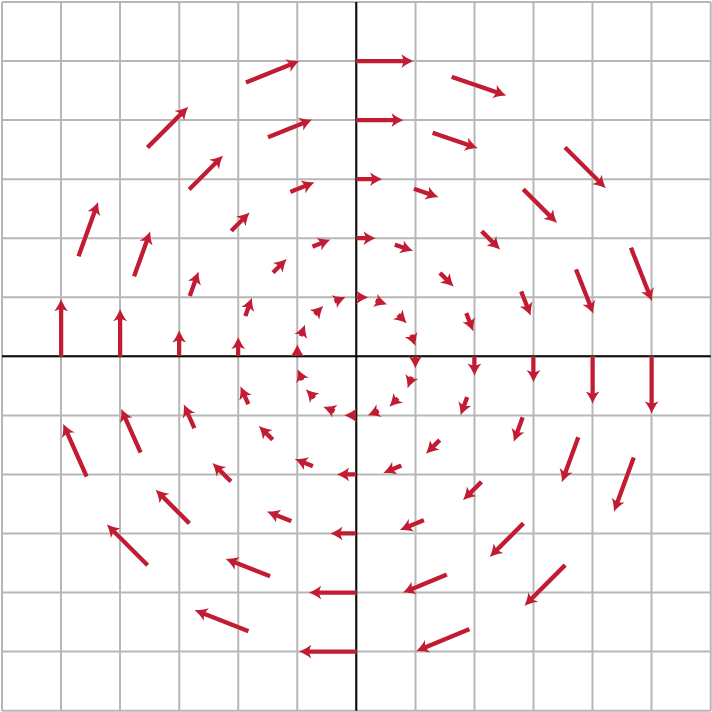
\includegraphics{6-campo-vectorial.png}
    \end{center}
    A partir del campo vectorial podemos ver que nuestra solución describe una circunferencia, es decir, conforme avanzamos en $t$ vamos a seguir \textit{dando vueltas} en una circunferencia fija.\\
\end{eg}
\section{Sistemas aut\'onomos en el plano.}
\begin{dfn}[Trayectoria del sistema]
    Una \textbf{trayectoria} del sistema $X' = F(X)$ es la curva que describe la solución, sin tener en cuenta la parametrización, es decir, es el subconjunto del plano descrito por la solución.
\end{dfn}
En general es más sencillo encontrar las trayectorias que resolver el sistema. Veamos un ejemplo:
\begin{eg}[Cálculo de las trayectorias de un sistema simple]
    Retomando el ejemplo anterior, consideramos el sistema:
    $$
        \mx{x\\y}' = \mx{y\\-x} = F(x, y)
    $$
    Las derivadas parciales son: $\dd{x}{t} = y$, $\dd{y}{t} = -x$, y afirmamos que:
    $$
        \dd{y}{x} "=" \frac{\dd{y}{t}}{\dd{x}{t}} = \frac{-x}{y}
    $$
    Que es la ecuación exacta $y \ dy + x\d x = 0$ con solución: $\frac{x^2+y^2}{2}=C$. Con lo que hemos hallado la ecuación que siguen las trayectorias de nuestro sistema original.
\end{eg}
En general, las trayectorias de:
\begin{gather*}
    x' = f(x, y)\\
    y' = g(x, y)
\end{gather*}
son las soluciones de $\dd{y}{x} = \frac{f(x, y)}{g(x, y)}$ siempre que $g(x, y) \neq 0$, o alternativamente, $\dd{x}{y} = \frac{g(x, y)}{f(x, y)}$ siempre que $f(x, y) \neq 0$. Por tanto, haremos lo primero cerca de puntos $(x, y)$ donde $g(x, y) \neq 0$ y lo segundo donde $f(x, y) \neq 0$.
\begin{dfn}[Punto crítico]
    Consideremos el sistema:
    \begin{gather*}
        x' = f(x, y)\\
        y' = g(x, y),\text{ con $f$, $g \in C^1$ en un abierto}
    \end{gather*}
    Un punto crítico (o de equilibrio) del sistema es un $(x_0, y_0)$ que cumple que $f(x_0, y_0) = g(x_0, y_0) = 0$.
\end{dfn}
\begin{obs}
    Sea $(x_0, y_0)$ un punto crítico, entonces:
    \begin{gather*}
        x(t) = x_0\\
        y(t) = y_0
    \end{gather*}
    es una solución del sistema y la trayectoria de  esa solución es el punto $x_0, y_0$.
\end{obs}
\begin{pro}[Soluciones con trayectorias iguales]
    Sea el sistema autónomo:
    $$
        \begin{cases}
            x' = f(x, y)\\
            y' = g(x, y)
        \end{cases}
    $$
    con $f, g \in \C^1(\Omega)$ y $\Omega$ un abierto de $\R^2$. Entonces:
    \begin{enumerate}
        \item \label{pro:trayeq-enum:1} Si $(x(t), y(t))$ es solución del sistema entonces:
        $$\begin{cases}
            \bar{x}(t) = x(t+a)\\
            \bar{y}(t) = y(t+a)
        \end{cases}$$
        también lo es y describe la misma trayectoria.
        \item Si dos soluciones describen la misma trayectoria, entonces están relacionadas como en \ref{pro:trayeq-enum:1}
    \end{enumerate}
\end{pro}
\begin{proof}
    Demostraremos cada apartado por separado, el primero es directo:
    \begin{enumerate}
        \item
        $$
            x'(t) = x'(t+a) = f(x(t+a), y(t+a)) = f(\bar{x}(t), \bar{y}(t))
        $$
        pues $f$ no depende de $t$. Entonces:
        $$
            f(t+a, x(t+a), y(t+a)) = f(t+a, \bar{x}(t), \bar{y}(t))
        $$
        \item Sabemos que $(x(t), y(t))$ y $(\bar{x}(t), \bar{y}(t))$ son dos soluciones con la misma trayectoria. Supongamos que $p = (x(0), y(0))$. Entonces $\exists a : (\bar{x}(a), \bar{y}(a)) = p$. Sea:
        $$
        \begin{cases}
            \hat{x}(t) = x(t+a)\\
            \hat{y}(t) = y(t+a)
        \end{cases}
        $$
        Entonces $(\hat{x}, \hat{y})$ es solución por \ref{pro:trayeq-enum:1}, y $(\hat{x}(0), \hat{y}(0)) = p = (x(0), y(0))$.\\
        Por unicidad, $\hat{x}(t) = x(t),\ \hat{y}(t) = y(t)$ en el intervalo del sistema y por tanto:
        $$
            \begin{cases}
                x(t) = \bar{x}(t+a)\\
                y(t) = \bar{y}(t+a)
            \end{cases}
        $$
    \end{enumerate}
\end{proof}
%%%%%%%%%%%%%%%%%%%%%%%%%%%%%%%%%%%%%%%%%%%%%%%%%%%%%%%%%%%%%%%% Clase del 02/04
Vamos a ver una versión del enunciado de existencia y unicidad en el caso de trayectorias, que se convierte en la siguiente proposición:
\begin{pro}[Existencia y unicidad de trayectorias]
    Sea $F\in C^1(\Omega)$, se tienen las siguientes alternativas para $2$ trayectorias de un sistema $\mathcal{S}$.
    \begin{enumerate}
        \item son disjuntas
        \item son la misma
    \end{enumerate}
\end{pro}
\begin{proof}
    Si $2$ trayectorias tienen un punto $p$ en común, entonces $p = X_1(t_0)$ para una solución $X_1$ de $\mathcal{S}$ y también $p = X_2(\bar{t}_0)$ donde $X_2$ es una solución de $\mathcal{S}$ que da lugar a la segunda trayectoria.\\
    Vimos que $\bar{X}_2(t) = X_2(t + \bar{t}_0 - t_0)$. Como $X_1$ y $\bar{X}_2$ son soluciones de $\mathcal{S}$ con dato inicial $X_1(t_0) = p = \bar{X}_2(t_0) = X_2(\bar{t_0})$.\\\\
    Por unicidad, $X_1 = \bar{X}_2$ y entonces dan lugar a las mismas trayectorias (aquí hemos usado que si $X(t)$ es solución de $\mathcal{S}$ también lo es $\bar{X}(t) = X(t+a)$, en este caso $a = \bar{t}_0 - t_0$.
\end{proof}
\begin{obs}
    Este resultado tiene relevancia cuando estamos en $\R^2$. Una curva en $R^2$ nos distingue dos regiones en el espacio. En general una trayectoria nos divide $\R^d$ en dos regiones disjuntas: $R_1,\ R_2$. Si tenemos una trayectoria $T$ que pase por $p \in R_i$ podemos asegurar que $T \subset R_i$.
\end{obs}
\begin{eg}[Trayectorias de la segunda Ley de Newton]\label{eg:tray-newt}
    La segunda ley de newton sigue la EDO $x'' = f(x)$. Vamos a transformarlo en un sistema:
    $$
        \begin{cases}
            x'' = f(x)\\
            y = x'
        \end{cases} \leadsto
        \begin{cases}
            x' = y\\
            y' = f(x)
        \end{cases}
    $$
    Una vez escrito el sistema, hallamos la ecuación de las trayectorias:
    $$
        \begin{cases}
            \dd{x}{t} = y(t)\\
            \dd{y}{t} = f(x(t))
        \end{cases}
    $$
    Para expresar la trayectoria tenemos que expresar $y = \text{funcion de } x$. Entonces:
    $$
        \dd{y}{x} =^{(*)} \dd{y}{t} \dd{t}{x} = \frac{\dd{y}{t}}{\dd{x}{t}} = \frac{f(x)}{y}
    $$
    (*) - Si $\dd{x}{t} \neq 0$\\
    Entonces:
    $$
        y\d y = f(x)\d x \leadsto \int y = \int f(x)
    $$
    Sea $U(x)$ una primitiva de $f(x)$, hallamos:
    $$
        \frac{y^2}{2} + U(x) = \text{ cte, que define $y$ implícitamente como función de $x$.}
    $$
    Con esto hemos hallado la expresión de un sistema conservativo:
    $$
        E_c + U = E
    $$
    Donde:
    \begin{enumerate}
        \item $E_c$ es la energía cinética con la unidad de masa $\equiv \frac{y^2}{2}$.
        \item $U$ es la energía potencial $\equiv U(x)$.
        \item $E$ es la energía del sistema, que permanece constante.
    \end{enumerate}
    A continuación, vamos a representar $U(x)$ frente a $x$, representaremos las trayectorias $y$ en función de $x$ y haremos un breve análisis de ellas y de los puntos críticos. Supongamos que la gráfica de $U(x)$ es la superior de la siguiente imagen.
    \begin{center}
        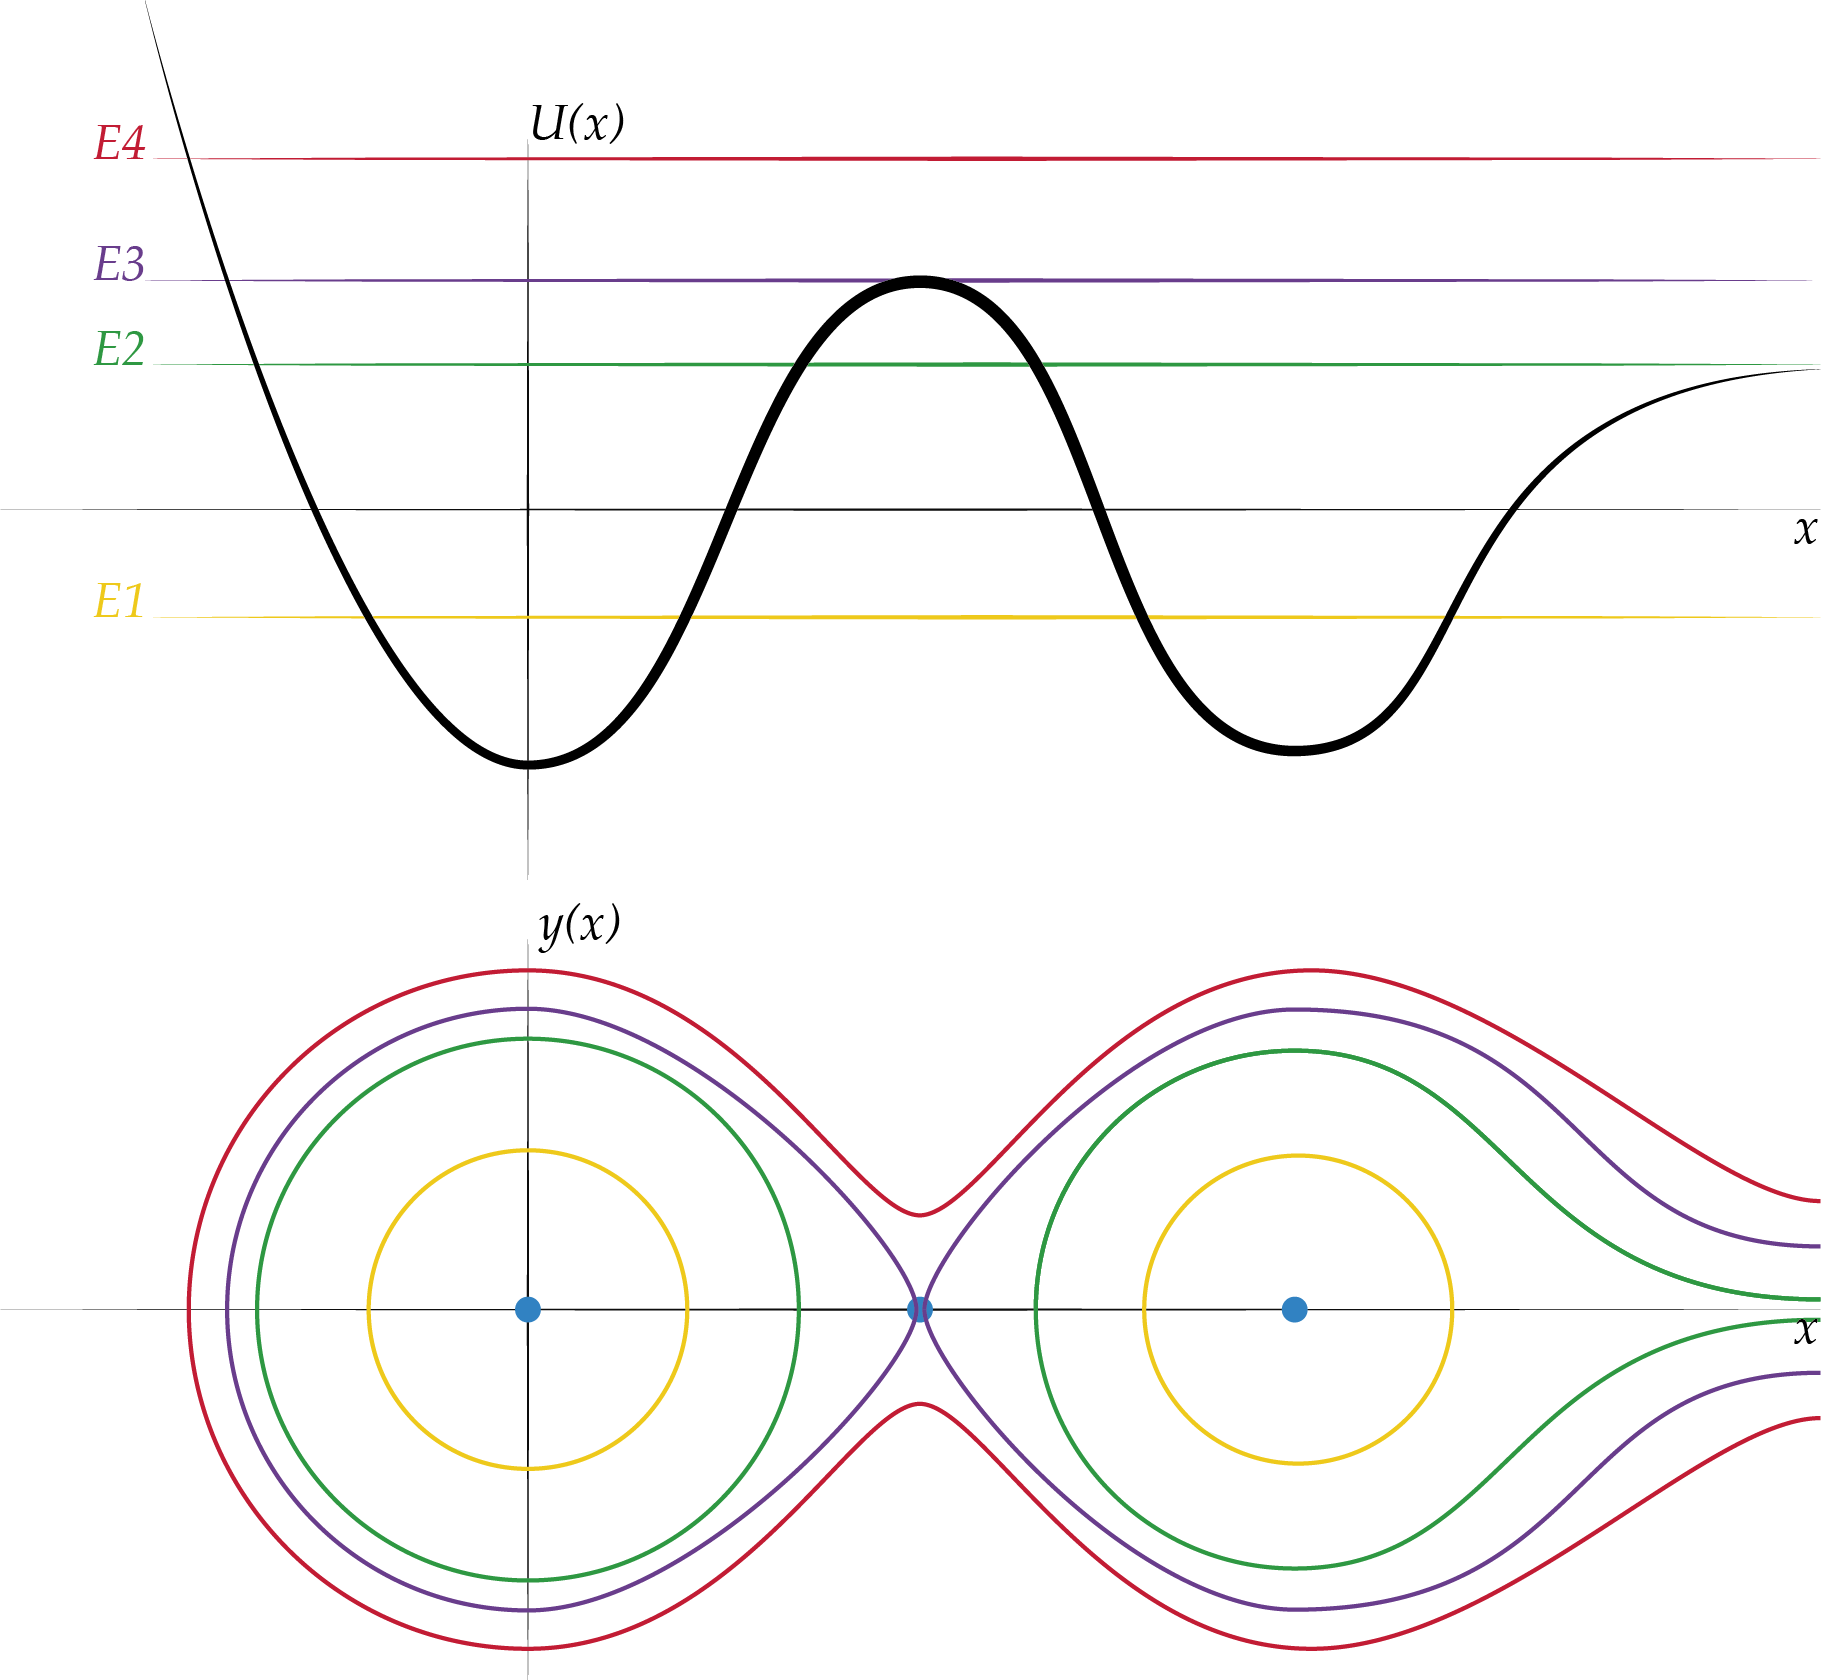
\includegraphics[width=0.5\textwidth]{6-ux-trayectorias.png}
    \end{center}
    Desarrollando la expresión anterior podemos despejar $y$ en función de $x$. Como $E_c = \frac{y^2}{2}$, entonces:
    $$
        y = \pm \sqrt{2(E_i - U(x))}
    $$
    es decir, la gráfica de $y$ frente a $x$ es función de la distancia de la gráfica de $U(x)$ a un nivel de energía fijo $E_i$, es por ello que cada nivel de energía $E_i$ da lugar a unas trayectorias distintas.\\
    El hecho de que las trayectorias sean cerradas no es trivial, si hacemos un análisis en profundidad de la expresión de $y$ frente a $x$ en los puntos en los que se anula $y$ veremos que su pendiente coincide, y por esto podemos afirmar que las dos partes definidas por el $\pm$ de la raíz \textit{unen bien}.\\\\
    % Representar U(x) frente a x
    % Representar las trayectorias finalmente
    % Explicar por qué unen bien las curvas.
    % Dar orientación a las Trayectorias
    % Dar explicación de puntos críticos
    Como el sistema es:
    $$
        \begin{cases}
            x' = y\\
            y' = f(x) = -U'(x)
        \end{cases}
    $$
    los puntos críticos son aquellos que cumplen $x' = 0, y' = 0$, es decir, aquellos valores $x_0$ que simultáneamente cumplen: $y(x_0) = 0$, $-U'(x_0) = 0$. Los hemos representado en la gráfica con un punto azul y se corresponden con aquellos valores de $x$ que hacen nula la derivada de $U(x)$.

    El valor $E_3$ toca un máximo de $U(x)$, sin embargo, por unicidad, la trayectoria que surge de este valor no puede tocar el punto crítico. Observamos que a partir de esta trayectoria se producen un cambio en la forma de las mismas. Si estamos en $\R^2$ llamaremos a este tipo de trayectorias \textbf{separatrices}.
\end{eg}

\begin{dfn}[Integral primera de un sistema]\label{dfn:iteg-prim}
    Una \textbf{integral primera} de un sistema es una función que es constante sobre cada solución o trayectoria.
\end{dfn}

\begin{obs}
    Vamos a hacer un comentario acerca del ejemplo \ref{eg:tray-newt}.
    \begin{itemize}
    \item Para ejemplificar la definición \ref{dfn:iteg-prim}, $\frac{y^2}{2} + U(x)$ es una integral primera del sistema:
    $$
    \begin{cases}
        x' = y\\
        y' = f(x) = -U'(x)
    \end{cases}
    $$
    En dimensión $2$ corresponde (esencialmente) a una ecuación implícita para las trayectorias y se pueden encontrar intentando resolver la EDO de las trayectorias:
    $$
    \dd{y}{x} = \frac{g(x, y)}{f(x, y)} \leadsto
    \begin{cases}
        x' = f\\
        y' = g
    \end{cases}
    $$
    En dimensiones más altas, una integral primera solo da una hipersuperficie en la que están las trayectorias o soluciones.
    Por ejemplo, en $\R^3$ sea el sistema:
    $$
    \begin{cases}
        x' = (...)\\
        y' = (...)\\
        z' = (...)
    \end{cases}
    $$
    Diremos que $h(x, y, z)$ es una integral primera $\iff h(x(t), y(t), z(t)) = cte$, es decir, la trayectoria es el conjunto $\{(x, y, z) \in \R^3 : h(x, y, z) = cte\}$. Ese conjunto es una superficie regular en los puntos en los que $\nabla h \neq 0$ (se puede despejar una variable en términos de las otras dos).
    \item En el ejemplo aparecen trayectorias cerradas. Veremos que corresponden a soluciones periódicas.
    \item También hemos visto que hay trayectorias que \textit{convergen} a un punto crítico (como la línea correspondiente a $E_3$ en el gráfico).\\
    Veremos que si $X(t)$ es una solución de $X' = F(x)$ y $X(t) \xrightarrow{t \to \pm \infty} p$, entonces $p$ es crítico. Basta que exista la sucesión $\{t_n\}_{n=1}^{\infty}$ tal que $X(t_n) \xrightarrow{n \to \infty} p$.
    \item Si ampliamos con un \textit{super-zoom} zonas del diagrama de fases, fuera del punto crítico se obtiene un gráfico como la zona azul de la siguiente imagen, que se corresponde a las tangentes a las trayectorias en esa zona; mientras que en un punto crítico obtenemos las otras dos. Se puede entender como el comportamiento lineal en esos puntos.
    \begin{center}
        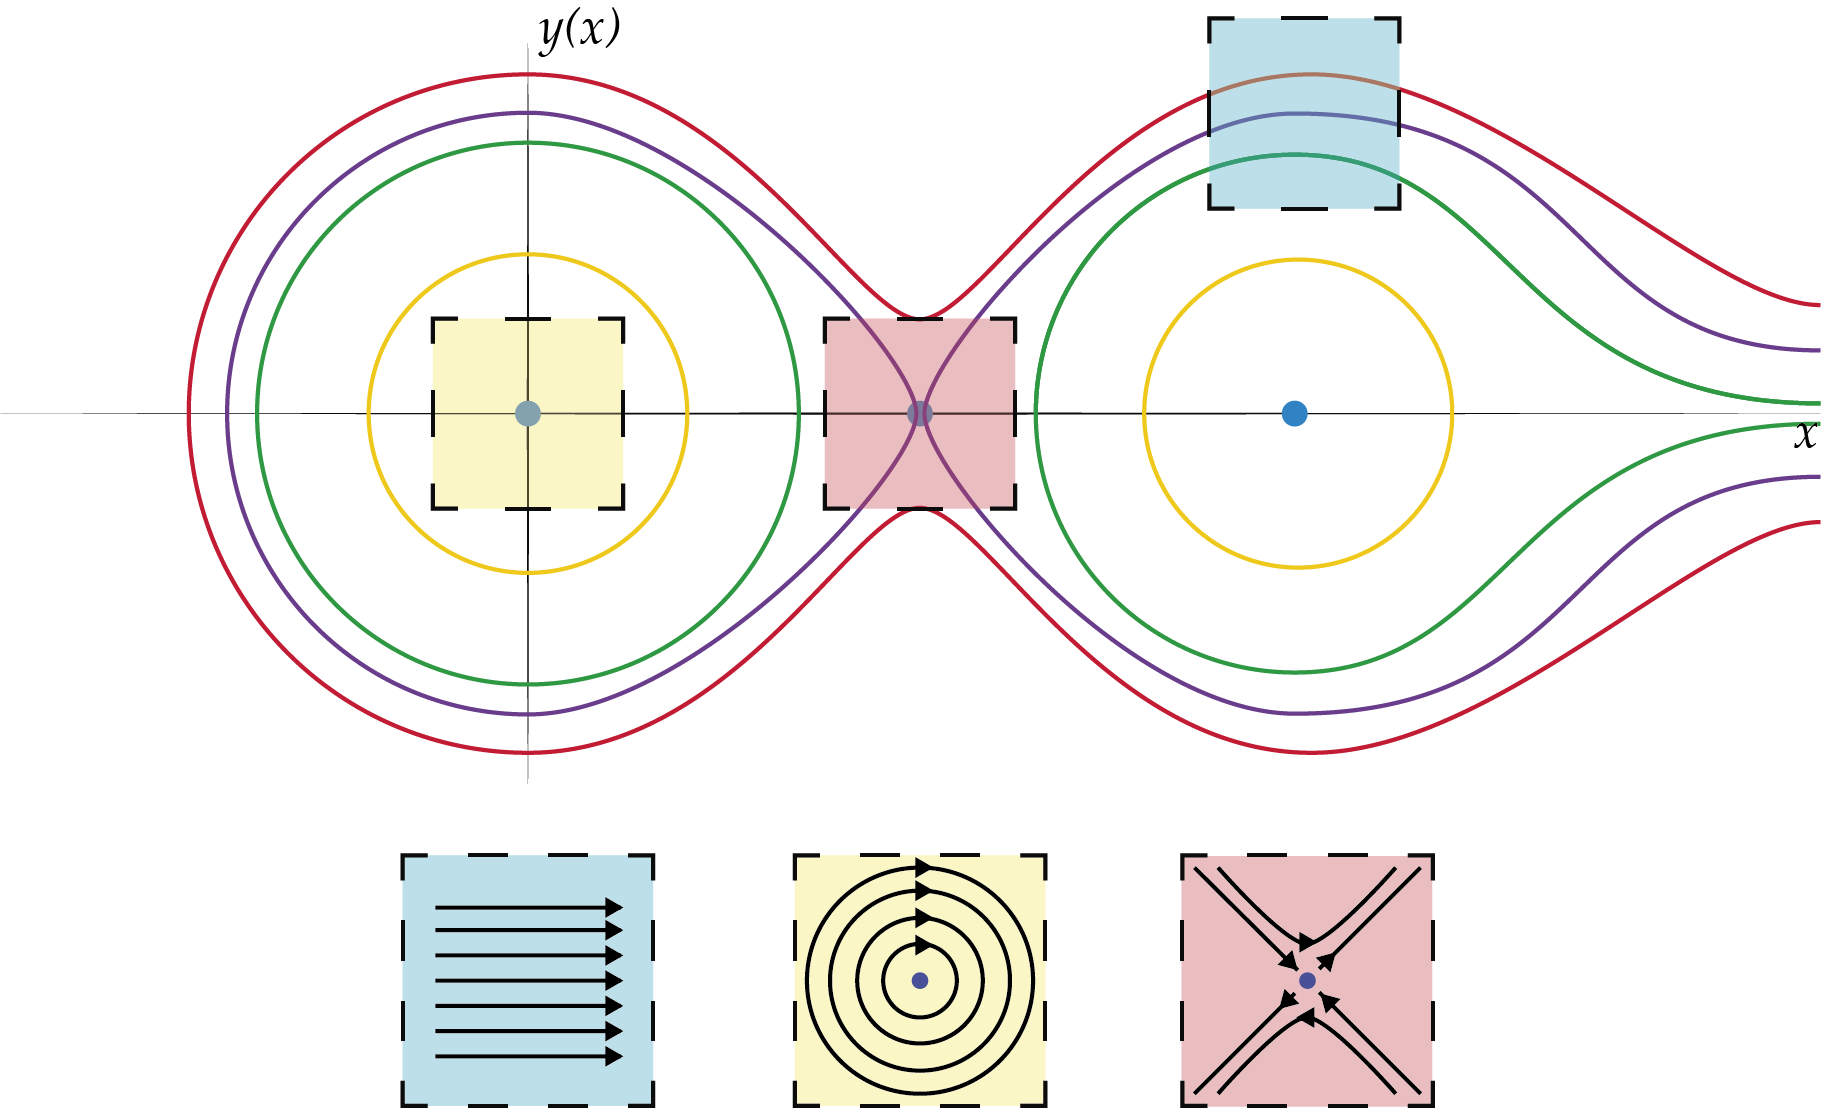
\includegraphics[width=0.5\textwidth]{6-trayectorias-zoom.png}
    \end{center}
    \end{itemize}
\end{obs}
\begin{th_ex}
    Sea el problema: $\theta '' = -\frac{g}{L} \sin(\theta)$, su representación como sistema es:
    $$
        \begin{cases}
            x = \theta\\
            y = \theta'
        \end{cases} \leadsto
        \begin{cases}
            x' = y\\
            y' = -\frac{g}{L}\sin(x)
        \end{cases}
    $$
    Y su diagrama de fases es:\\\\
    \begin{center}
        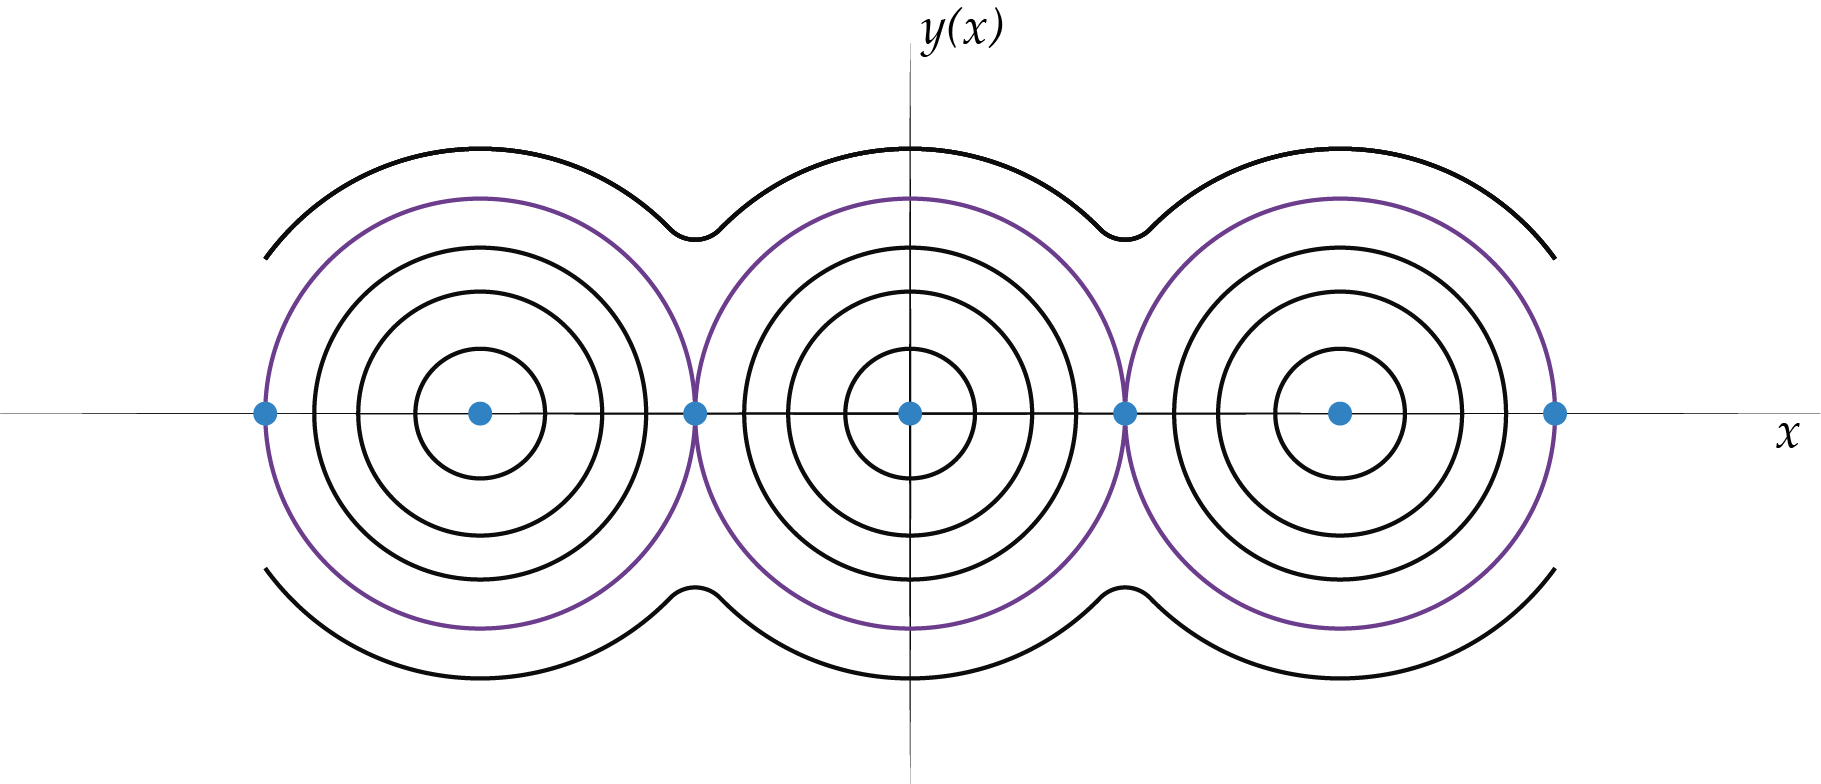
\includegraphics[width=0.5\textwidth]{6-trayectorias-pendulo.png}
    \end{center}
    \begin{itemize}
        \item Comprueba que la figura se corresponde con su diagrama de fases.
        \item ¿Cuáles son los puntos críticos marcados?
        \item Da dirección a las trayectorias.
    \end{itemize}
\end{th_ex}
\subsection{Sistemas conservativos en dimensión mayor que 1}
\begin{dfn}[Sistema conservativo]
    Consideramos el sistema que surge de la EDO $X'' = F(X)$, con $F: \Omega \to \R^d$, $U: \Omega \to \R$ regular.\\
    Diremos que el sistema es un \textbf{sistema conservativo} cuando $F = -\nabla U$.
\end{dfn}
\begin{pro}
    Sea el sistema $X'' = F(X)$ conservativo, entonces:
    $$
        \frac{||X'(t)||_2^2}{2} + U(X(t)) = cte, \text{ es decir, } \frac{||y||_2^2}{2} + U(x) \text{ es integral primera}
    $$
\end{pro}
\begin{proof}
    $$
    \Dd{t} \left(\frac{||X'(t)||_2^2}{2} +  U(X(t)\right) = \frac{2 X' \cdot X''}{2} + (\nabla U(X(t))) \cdot X'(t) = X'(X'' + \nabla U(X(t))) = X'(X'' - F(X(t))) = 0
    $$
\end{proof}
%%%%%%%%%%%%%%%%%%%%%%%%%%%%%%%%%%%%%%%%%%%%%%%%%%%%%%%%%%%%%%%% Clase del 04/04
\begin{eg}[Trayectorias de un pozo doble]
    Sea la EDO $x'' = x - x^3 = f(x)$. Como viene siendo habitual en sistemas mecánicos, $f(x) = -U'(x)$ y por tanto $U(x) = -\frac{x^2}{2}+\frac{x^4}{4}$. Entonces nuestro sistema es:
    $$
    \begin{cases}
        x' = -\frac{x^2}{2}+\frac{x^4}{4}\\
        y' = x - x^3 = -U'(x)
    \end{cases}
    $$
    Como los puntos críticos cumplen $y=0,\ y'= x(1-x^2) = 0$, entonces: $x=0,\ x=\pm 1$. Por tanto, los puntos críticos son: $ (-1, 0),\ (0, 0),\ (1, 0)$.\\
    Sabemos que $\frac{y^2}{2} + U(x)$ se conserva en las trayectorias, es decir, las trayectorias están descritas por $\frac{y^2}{2}  -\frac{x^2}{2}+\frac{x^4}{4} = cte$ (notamos que es la integral de $y' = -U'(x)$). Por tanto, fijando distintas constantes hallamos el gráfico de las trayectorias:
    \begin{center}
        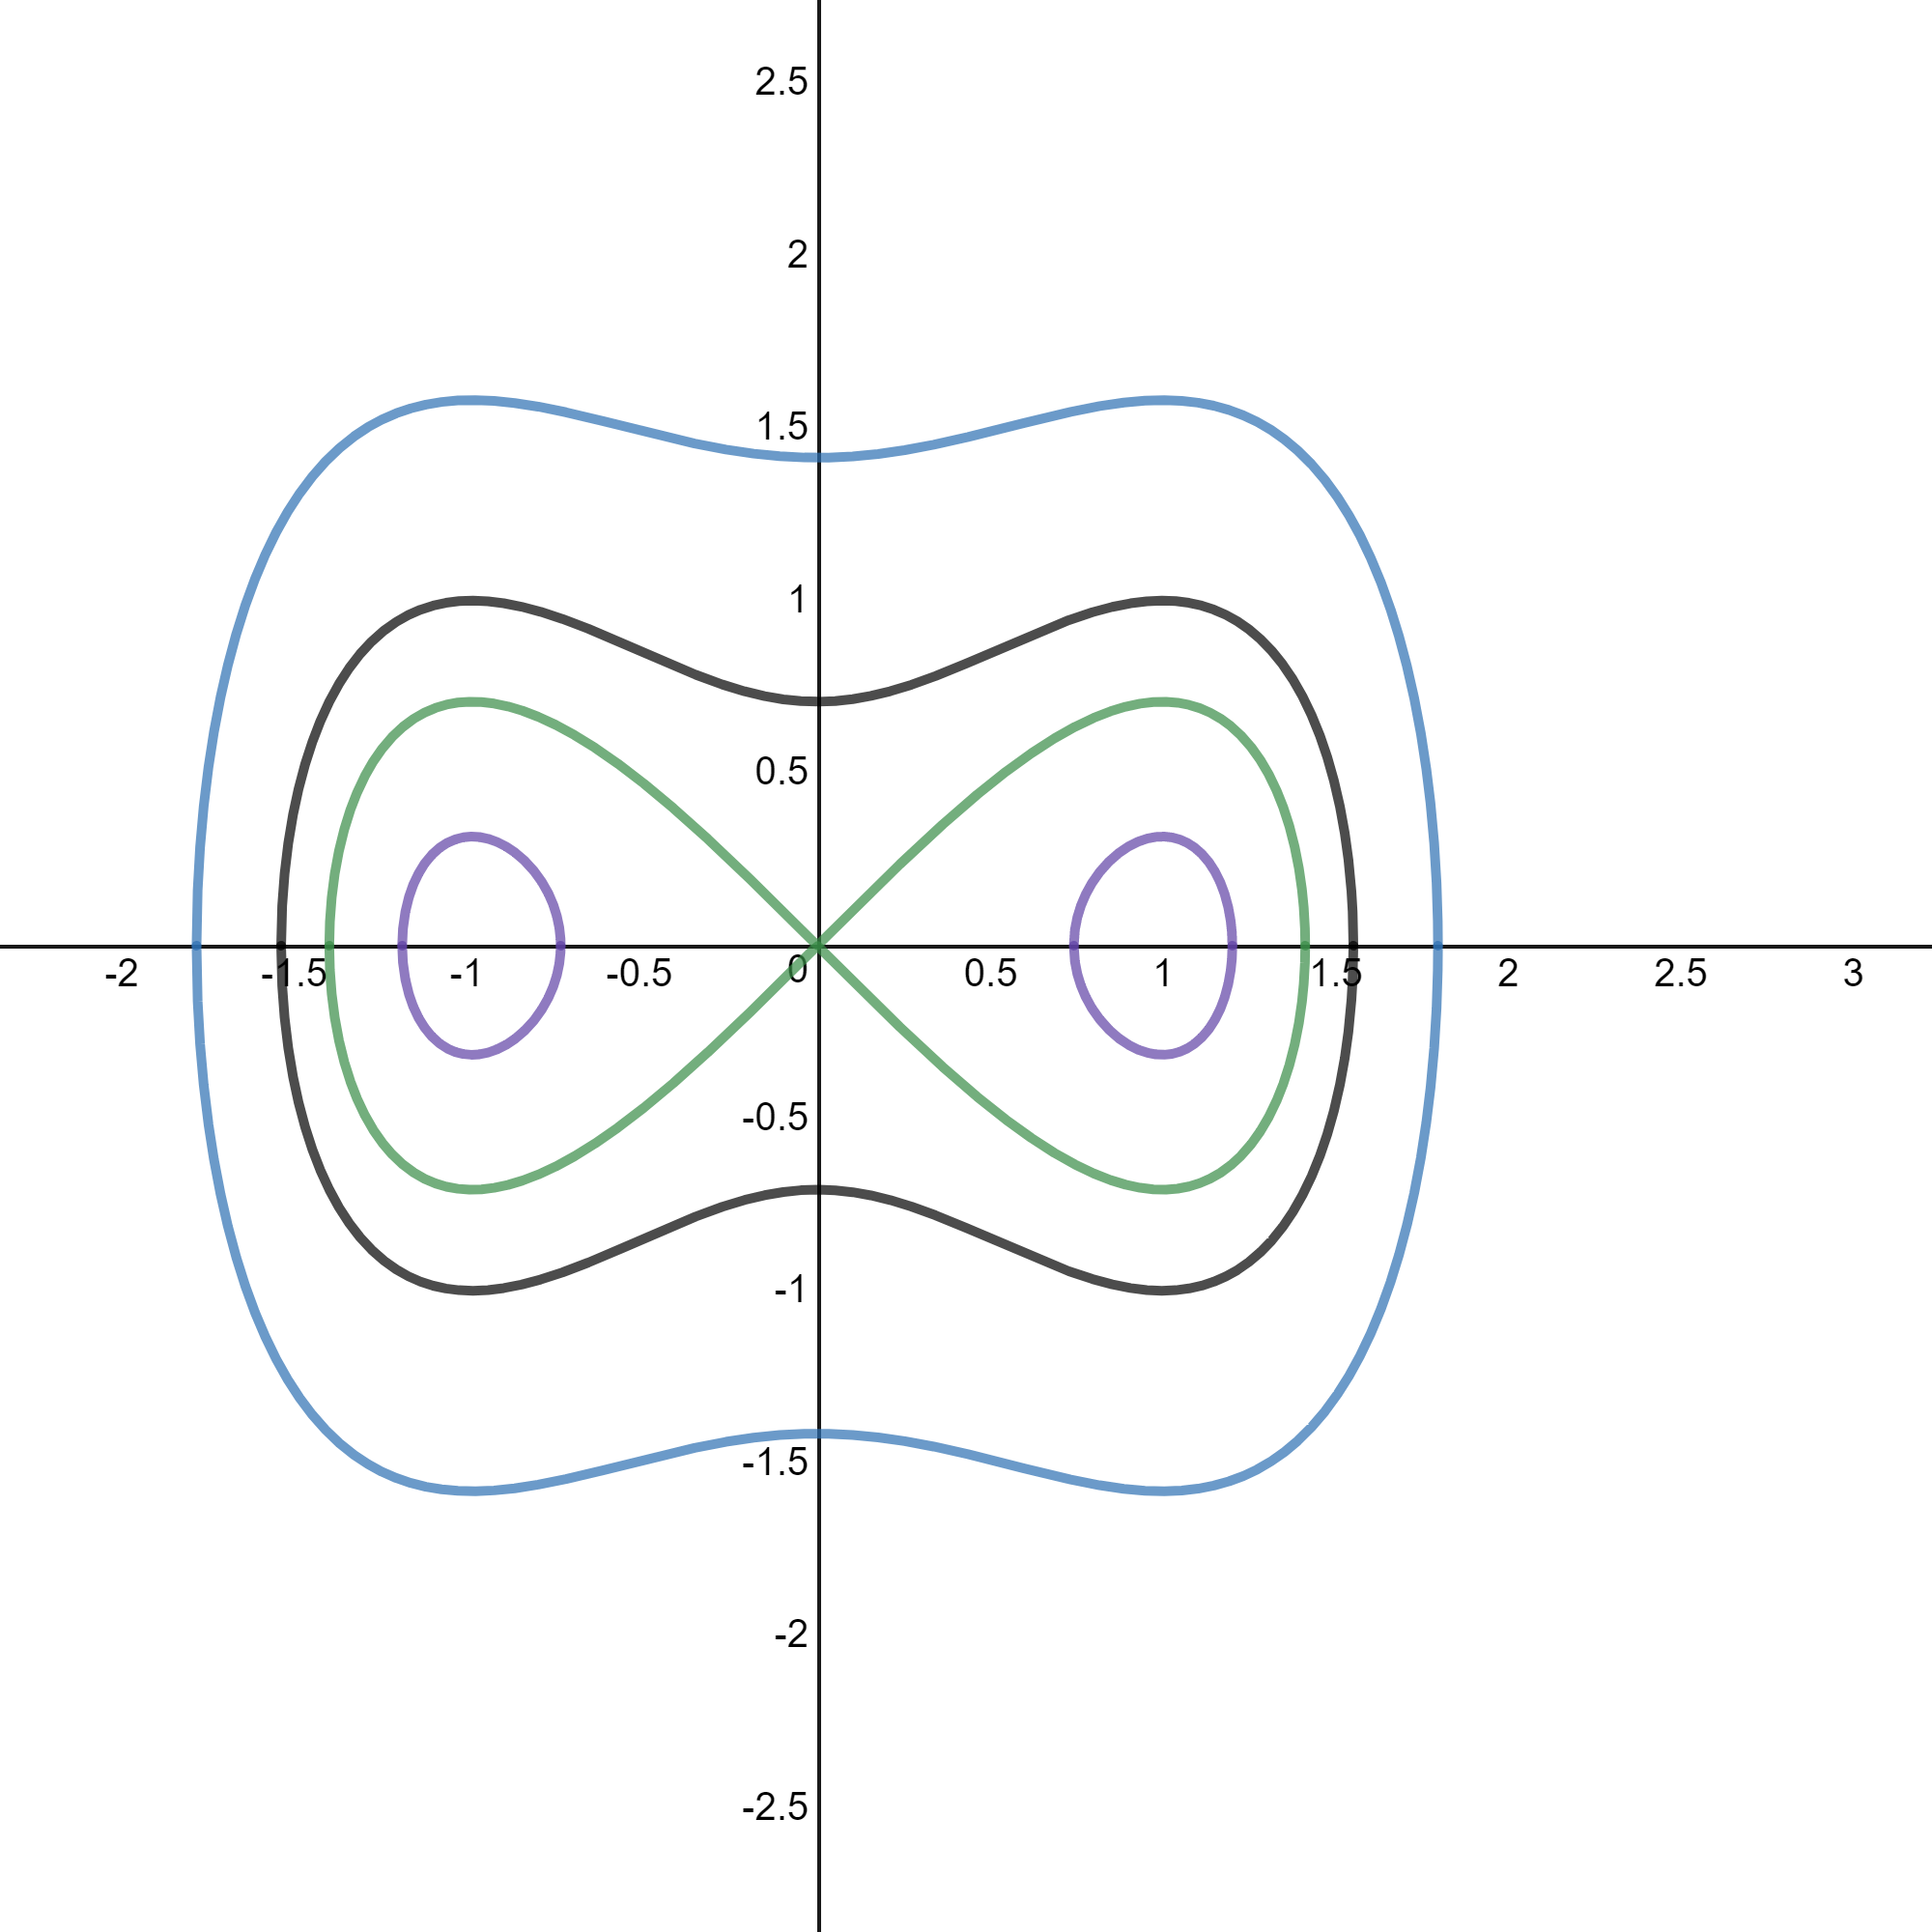
\includegraphics[width=0.5\textwidth]{6-pozo-doble.png}
    \end{center}
\end{eg}
\begin{obs}
    La simetría con respecto al eje X tiene que ver con reversibilidad en $t$, es decir, si $x(t)$ es solución de la EDO, entonces $\bar{x}(t) = x(-t)$ también lo es.
\end{obs}
\begin{pro}
Sea $X'=F(X)$ con $F\in C^1(\Omega)$ y $\Omega$ abierto en $\R^d$. Si $X(t)$ es una solución que da lugar a una trayectoria cerrada, entonces es periódica.
\end{pro}
\begin{proof}
    Dividiremos la prueba en distintos pasos:
    \begin{enumerate}
        \item Si la trayectoria $X(t)$ es cerrada, entonces por definición $\exists t_1 < t_2 : X(t_1) = X(t_2)$.
        \item Sea $T = t_2 - t_1$ y sea $\bar{X}(t) = X(t+T)$ entonces $\bar{X}$ es una solución del sistema, pues $\bar{X}'(t) = X'(t + T) = F(X(t + T)) = F(\bar{X}(t))$.\\
        Por otro lado, $\bar{X}(t_1) = X(t_1 + t_2 - t_1) = X(t_2) = X(t_1)$, es decir, $X, \bar{X}$ resuelven el PVI:
        $$
        \begin{cases}
            Y' = F(Y)\\
            Y(t_1) = X(t_1) = \bar{X}(t_1)
        \end{cases}
        $$
        y por unicidad $\bar{X} = X$.
    \end{enumerate}
\end{proof}
\begin{th_ex}
    Demostrar que si $X(t) \neq cte$ (es decir, su trayectoria no es un punto crítico), entonces $X$ tiene un periodo mínimo.
\end{th_ex}
\section{Linealizaci\'on y clasificaci\'on de puntos cr\'iticos}
Supongamos que tenemos un sistema como:
$$
    \begin{cases}
        x' = f(x, y)\\
        y' = g(x, y)
    \end{cases}
$$
y supongamos además que $(x_0, y_0)$ es un punto crítico, es decir, $f(x_0, y_0) = g(x_0, y_0) = 0$. Vamos a \"ampliar\" el gráfico de las trayectorias lo suficiente como para aproximar las tangentes a la trayectorias. Hacer esto formalmente es aproximar por Taylor.
$$
    f(x, y) = f(x_0, y_0) + f_x(x_0, y_0)(x-x_0) + f_y(x_0, y_0)(y-y_0) + R(x, y)
$$
donde (supongamos que $f \in C^2$): $ R(x, y) \text{ es } R(x, y) = O((x-x_0)^2 + (y-y_0)^2)$. Para simplificar nuestro resultado, hacemos el cambio $u = x-x_0$ y $v = y-y_0$, con lo que obtenemos:
\begin{gather*}
    u' = au + bv + O(u^2+v^2)
\end{gather*}
Haciendo lo mismo con $g$, obtenemos:
$$
    v' = cu + dv + O(u^2 + v^2)
$$
Donde
    \begin{gather*}
        a = f_x(x_0, y_0)\\
        b = f_y(x_0, y_0)\\
        c = g_x(x_0, y_0)\\
        d = g_y(x_0, y_0)
    \end{gather*}
Este sistema es aproximadamente (si $|u|<<1$ y $|v|<<1$):
$$
    \begin{cases}
        u' = au + bv\\
        v' = cu + dv
    \end{cases} \text{ y lo denominamos sistema linealizado en el punto crítico}
$$
Vamos a suponer que:
$$
    \mx{a &b\\ c &d} \neq 0\text{, es decir, el punto crítico es \textit{no degenerado}.}
$$
Esto tiene como consecuencia que el punto crítico es aislado, es decir, en un entorno de $(x_0, y_0)$ no hay otro punto crítico.
Sea $H$ la función que aplica: $(x, y) \to (f(x, y), g(x, y))$, si el punto es aislado entonces: $det(DH(x_0, y_0)) \neq 0$, es decir, $H$ es invertible cerca de $(x_0, y_0)$. Está claro que $u=0, v=0$ es el único punto crítico del sistema lineal:
$$
    \begin{cases}
        u' = au + bv\\
        v' = cu + dv
    \end{cases}
$$
y vamos a estudiar cómo son sus trayectorias.
%%%%%%%%%%%%%%%%%%%%%%%%%%%%%%%%%%%%%%%%%%%%%%%%%%%%%%%%%%%%%%%% Clase del 08/04
\subsection{Clasificaci\'on de puntos cr\'iticos}
Sea el sistema lineal:
$$
    \mathcal{S} \equiv \begin{cases}
        x' = f(x, y)\\
        y' = g(x, y)
    \end{cases}
$$
y sea $(x_0, y_0)$ un punto crítico.
\begin{dfn}[Punto crítico estable]
    Diremos que $(x_0, y_0)$ es un punto crítico estable si y sólo si:\\
    $\forall \varepsilon > 0, \exists \delta > 0 :$  si  $(x(t), y(t))$  es solución de  $\mathcal{S}$, con $(x(t_0), y(t_0)) \in \B((x_0, y_0), \delta)$ entonces $(x(t), y(t))$ existe $\forall t \geq t_0$ y $(x(t), y(t)) \in \B((x_0, y_0), \varepsilon)$
\end{dfn}
\begin{dfn}[Punto crítico asintóticamente estable.]
    Diremos que $(x_0, y_0)$ es un punto crítico asintóticamente estable si y sólo si:\\
    $\exists \delta > 0 : $ si  $(x(t), y(t))$  es solución de  $\mathcal{S}$, con $(x(t_0), y(t_0)) \in \B((x_0, y_0), \delta)$ entonces $(x(t), y(t))$ existe $\forall t \geq t_0$ y converge a $(x_0, y_0)$.
\end{dfn}
Vamos a desarrollar la clasificación de distintos puntos críticos.\\
Sea el sistema:
$$
    \mathcal{SI} \equiv \mx{x'\\y'} = \mx{a & b\\ c & d} \mx{x \\ y}
$$
con $\A = \mx{a & b\\ c & d}$ invertible. El único punto crítico es $(0, 0)$.
Vamos a clasificarlo:
\begin{enumerate}
    \item Caso de autovalores reales:\\
    Sean $\lambda_1,\ \lambda_2$ los autovalores de $\A$.
    \begin{enumerate}
        \item $\lambda_1 \neq \lambda_2$.\\
        Si $V_j$ es autovector de $\lambda_j$, $V_1, V_2$ forman una base.\\
        las soluciones de $\mathcal{SI}$ son:
        $$
            \alpha_1 e^{\lambda_1t}V_1 + \alpha_2 e^{\lambda_2t}V_2
        $$
        Pasamos a coordenadas $(z, w)\in\R^2$ tal que:
        $$
            \mx{x\\y} = z V_1 + wV_2, \text{ es decir, cambio de base de $\{e_1, e_2\}$ a $\{V_1, V_2\}$}
        $$
        En esas coordenadas las soluciones son:
        $$
            \begin{cases}
                z = \alpha_1 e^{\lambda_1 t}\\
                w = \alpha_2 e^{\lambda_2 t}
            \end{cases}
        $$
        \begin{enumerate}
            \item $\lambda_2 > \lambda_1 > 0$.\\
            Digamos que $\alpha_1, \alpha_2 > 0 \implies z, w > 0$. Entonces las trayectorias son:
            $$
                w = \alpha_2 e^{\lambda_2 t} = \alpha_2 \left(e^{\lambda_1 t }\right)^{\sfrac{\lambda_2}{\lambda_1}} = \alpha_2 \left(\frac{z}{\alpha_1}\right)^{\sfrac{\lambda_2}{\lambda_1}}
            $$ es decir, $w \equiv C z^{\sfrac{\lambda_2}{\lambda_1}}$ y $\frac{\lambda_2}{\lambda_1} > 1$. Podemos representarlas en las variables $z, w$, lo que nos da como resultado un punto \textbf{inestable}:\\
            \begin{center}
                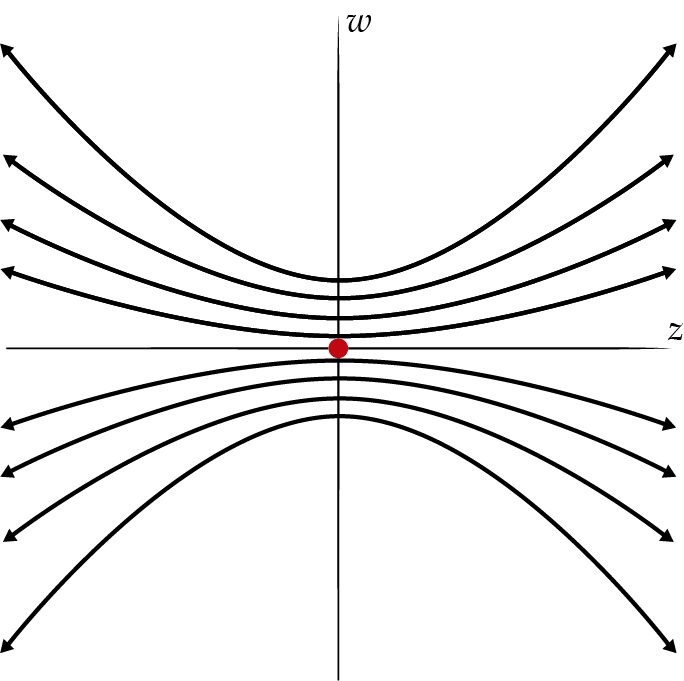
\includegraphics[width=0.5\textwidth]{6-nodo-inestable.png}
            \end{center}
            Si quisiéramos representarlas en las variables originales $x, y$ tendríamos que deshacer el cambio. $V_2$ es el autovector que corresponde al autovalor de mayor tamaño $|\lambda_2|$.\\\\
            Las trayectorias son tangentes a la recta de autovector con autovalor $\lambda_i$ con valor absoluto más bajo, en este caso $\lambda_1$.
            %%TODO: Añadir representación gráfica
            \item $\lambda_2 < \lambda_1 < 0$.
            El desarrollo del apartado anterior nos sirve para este caso también, es decir, las trayectorias siguen siendo:
            $$
                w = C (z)^{\sfrac{\lambda_2}{\lambda_1}},\ \frac{\lambda_2}{\lambda_1} > 1.
            $$
            Y su representación gráfica sería un punto \textbf{asintóticamente estable}:
            \begin{center}
                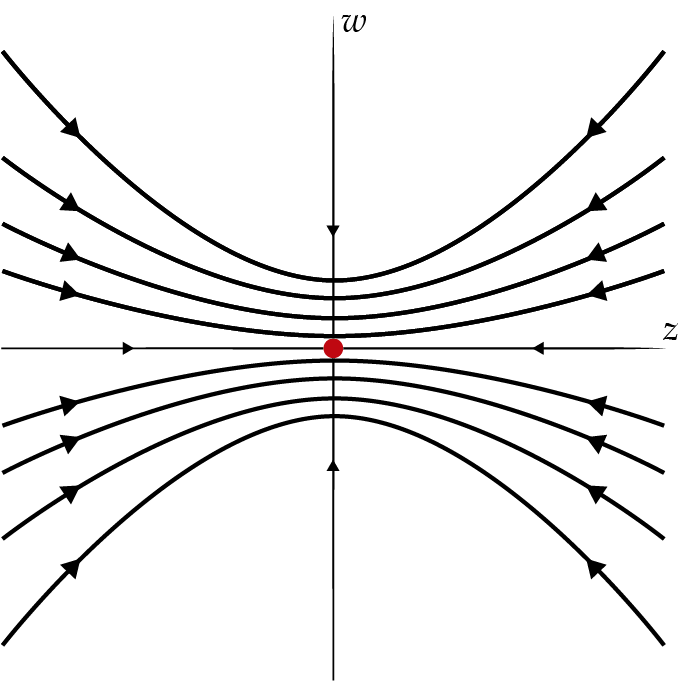
\includegraphics[width=0.5\textwidth]{6-nodo-estable.png}
            \end{center}
            Las trayectorias son tangentes a la recta de autovector con autovalor $\lambda_i$ con valor absoluto más bajo, en este caso $\lambda_1$.
            \item $\lambda_1 < 0 < \lambda_2$.
            Entonces $z = \alpha_1 e^{\lambda_1t} \downarrow 0$ cuando $t\to\infty$, y $w = \alpha_2 e^{\lambda_2t} \uparrow \infty$ cuando $t\to\infty$. Entonces el punto crítico es un \textbf{punto de silla} y sus trayectorias son:
            \begin{center}
                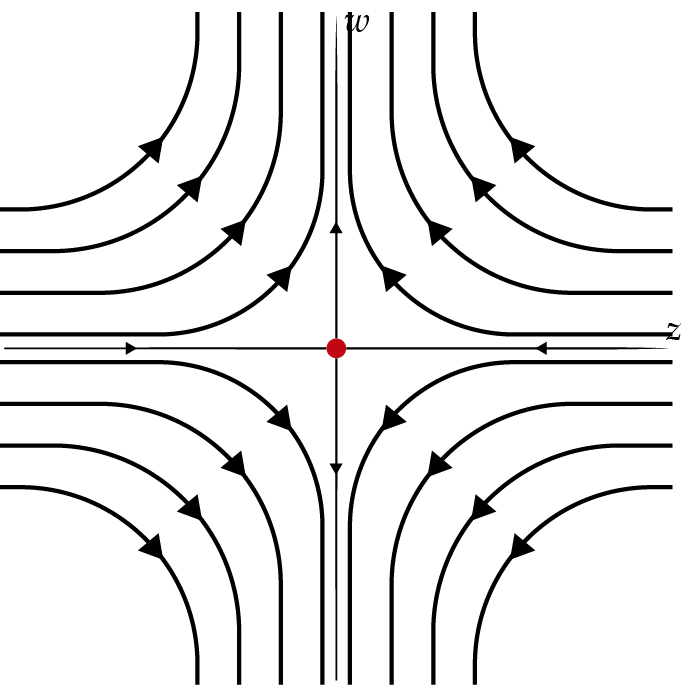
\includegraphics[width=0.5\textwidth]{6-punto-de-silla.png}
            \end{center}
        \end{enumerate}
        \item $\lambda_1 = \lambda_2 \neq 0$.
        Ahora no tenemos garantías de tener 2 autovectores independientes.
        \begin{enumerate}
            \item $\exists V_1, V_2$ autovectores independientes. En este caso es:
            $$
            \begin{cases}
                z = \alpha_1 e^{\lambda t}\\
                x = \alpha_2 e^{\lambda t}
            \end{cases}
            $$
            Entonces, dependiendo del signo de $\lambda = \lambda_1 = \lambda_2$ tendremos un \textbf{punto crítico inestable} $\lambda > 0$ o asintóticamente estable $\lambda < 0$.
            \begin{center}
                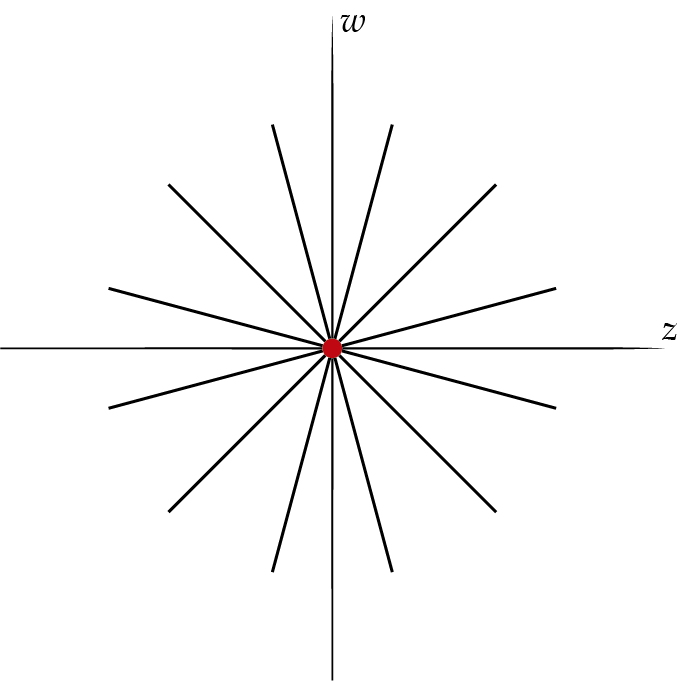
\includegraphics[width=0.5\textwidth]{6-autovalores-iguales-1.png}
            \end{center}
            \item $\not\exists V_1, V_2$ autovectores independientes, es decir, la dimensión del subespacio de autovectores es 1.\\
            Sea $V_1$ el autovector que encontramos, entonces la base de las soluciones es:
            $$
                e^{\lambda t} V_1,\ e^{\lambda t}(V_2 + t V_1)
            $$
            Donde $V_2$ es un autovector generalizado, es decir, $(\A - \lambda I)V_2 = V_1$.
            Entonces la solución general es:
            $$
                ae^{\lambda t} V_1 + b  e^{\lambda t}(V_2 + t V_1) = (a+bt)e^{\lambda t}V_1 + be^{\lambda t}V_2
            $$
            $V_1, V_2$ forman una base de $\R^2$, y en coordenadas $z, w$:
            $$
                \mx{x \\ y } = z V_1 + w V_2
            $$
            Vamos a representar las trayectorias $x, y$ para distintos casos, siempre con $\lambda > 0$.\\
            \begin{itemize}
                \item $b = 0 \leadsto z = ae^{\lambda t},\ w = 0$.
                \item $ b = 1, a = 0 \leadsto z = te^{\lambda t},\ w = e^{\lambda t}$. Y su representación muestra un \textbf{nodo degenerado inestable} (si $\lambda < 0$ tendríamos un nodo degenerado asintóticamente estable).
                \begin{center}
                    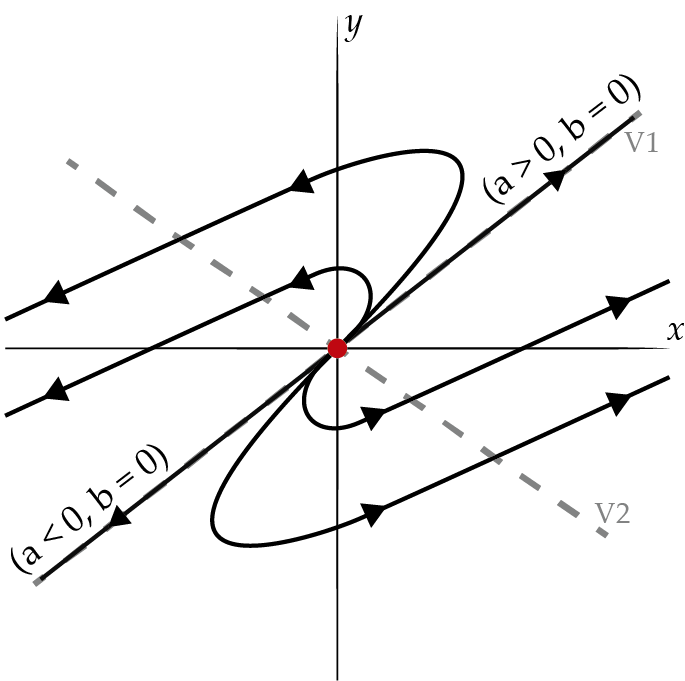
\includegraphics[width=0.5\textwidth]{6-autovalores-iguales-2.png}
                \end{center}
            \end{itemize}
            %%%%%%%%%%%%%%%%%%%%%%%%%%%%%%%%%%%%%%%%%%%%%%%% Clase del 09/04
        \end{enumerate}
    \end{enumerate}
    \item Caso autovalores complejos.\\
    Tendremos $\lambda \pm = \alpha \pm i \beta$, con $\beta > 0$. Llamaremos $\lambda$ a $\lambda = \alpha \mbf{+} i\beta$.
    \begin{enumerate}
        \item $\Re(\lambda) = 0$, es decir $\alpha = 0$ y $\lambda \pm$ son imaginarios puros.\\
        Entonces, $\lambda = \alpha + i\beta$ tiene como autovector $W = V_1 + iV_2$ y $\lambda\mbf{-} = \alpha - i\beta$ tiene como autovector $\bar{W} = V_1 - i V_2$.\\
        Su solución general es:
        $$
            a Re(e^{i\beta t} W) + b Im(e^{i \beta t} W)
        $$
        Y como:
        $$
            e^{i\beta t} W = \cos(\beta t) V_1 - \sin(\beta t)V_2
        $$
        podemos reescribir la solución general como:
        $$
            (a \cos(\beta t) + b \sin(\beta t))V_1 + (b \cos(\beta t) - a \sin(\beta t))V_2
        $$
        Por tanto, en coordenadas $z, w$:
        $$
            \begin{cases}
                z = a \cos(\beta t) + b \sin(\beta t)\\
                w = b \cos(\beta t) - a \sin(\beta t)
            \end{cases}
        $$
        Esto quiere decir que como $z^2 + w^2 = a^2 + b^2$ , tenemos círculos de radio $\sqrt{a^2+b^2}$. En $x, y$ serían elipses. Su representación geométrica da lugar a un \textbf{centro} (que es estable).
        \begin{center}
            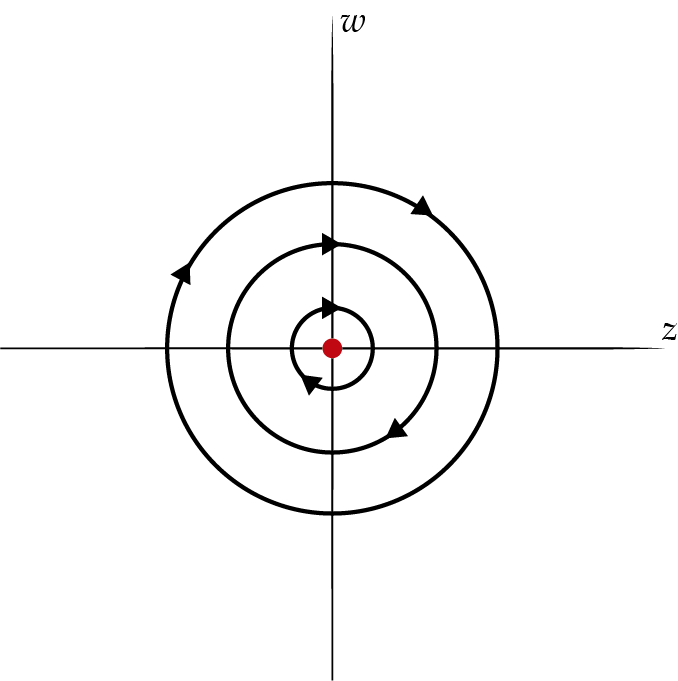
\includegraphics[width=0.5\textwidth]{6-centro.png}
        \end{center}
        Es fácil ver que si cambia el signo de $\beta$, cambia el sentido de las trayectorias.
        \item $Re(\lambda \neq 0)$.\\
        Repitiendo el mismo cálculo que en la sección anterior, esta vez con la solución general:
        $$
            a Re(e^{\alpha t} e^{i\beta t} W) + b Im(e^{\alpha t}e^{i \beta t} W)
        $$
        Obtendríamos en coordenadas $z, w$:
        $$
            \begin{cases}
                z = e^{\alpha t} (a \cos(\beta t) + b \sin(\beta t))\\
                w = e^{\alpha t} (b \cos(\beta t) - a \sin(\beta t))
            \end{cases}
        $$
        Y su representación en $z, w$ da lugar a una espiral. Representamos dos casos, con $\alpha > 0$ obtenemos una espiral inestable, y con $\alpha < 0$ una espiral asintóticamente estable. De nuevo, $\beta$ da el sentido del giro.
        \begin{center}
            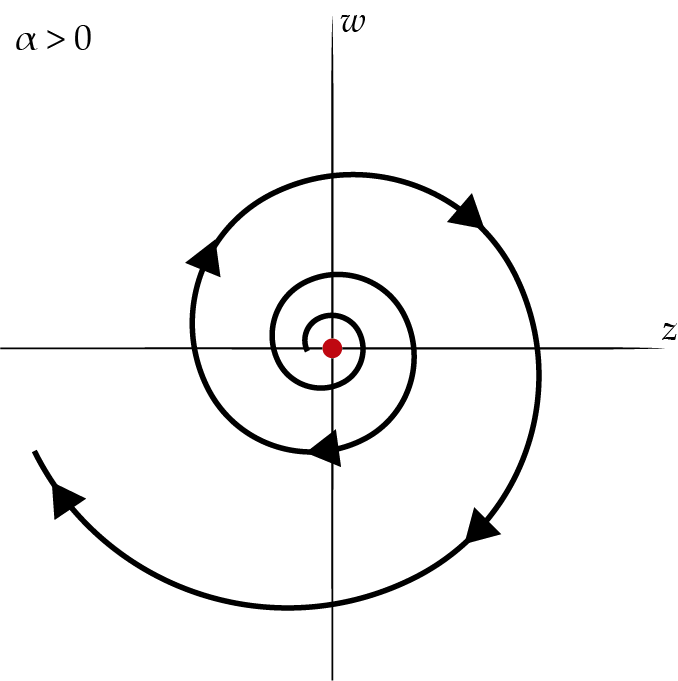
\includegraphics[width=0.4\textwidth]{6-espiral-inestable.png}
            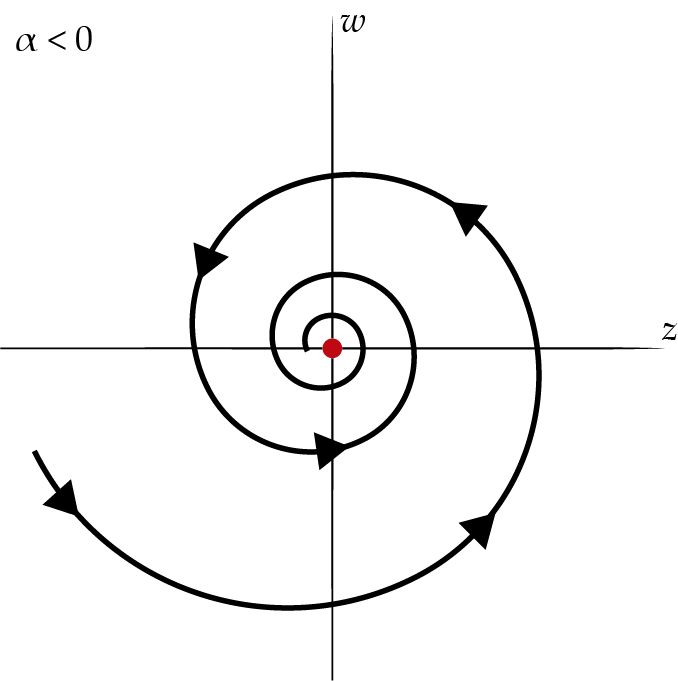
\includegraphics[width=0.4\textwidth]{6-espiral-estable.png}
        \end{center}
    \end{enumerate}
\end{enumerate}
\subsubsection{Criterios para distinguir puntos cr\'iticos}
Sin embargo, lo que hemos visto en la sección anterior puede resultar tedioso, por lo que vamos a ver otra forma de distinguir los diferentes casos utilizando la traza y el determinante de la matriz: $\A = \mx{a & b \\ c & d}$.\\
Es claro que los autovalores $\lambda_i$ siguen la ecuación:
$$
    \lambda^2 - (a+d) \lambda + (ad - bc) = 0
$$
o lo que es lo mismo, sea $T = \mathrm{traza}(\A)$ y $D = \mathrm{det}(\A)$ entonces la ecuación es:
$$
    0 = \lambda^2 - T\lambda + D = (\lambda - \lambda_1)(\lambda - \lambda_2)\text{, es decir:}
$$
$$
    \begin{cases}
        T = \lambda_1 + \lambda 2\\
        D = \lambda_1 \lambda_2
    \end{cases}
$$
\begin{pro}[Clasificación de puntos críticos en función del determinante y la traza]
    Sea el sistema:
    $$
        \mathcal{SI} \equiv \mx{x'\\y'} = \mx{a & b\\ c & d} \mx{x \\ y},\ \A = \mx{a & b \\ c & d}
    $$
    y sea $T = \mathrm{traza}(\A)$ y $D = \mathrm{det}(\A)$ entonces:
    \begin{itemize}
        \item $T^2 - 4D < 0 \implies$ los autovalores son complejos. \textbf{Espirales}.
        \item $T^2 - 4D < 0$ y $T = 0 \implies$ los autovalores son complejos con $Re(\lambda) = 0$. \textbf{Centros}.
        \item $T^2 > 4D \implies$ autovalores reales y distintos. \textbf{Nodos}.
        \item $D < 0 \implies$ autovalores reales con distinto signo. \textbf{Puntos de silla}.
        \item $T^2 = 4D \implies$ autovalores reales iguales. \textbf{Nodos degenerados}.
    \end{itemize}
    El siguiente dibujo resume lo visto:
    \begin{center}
        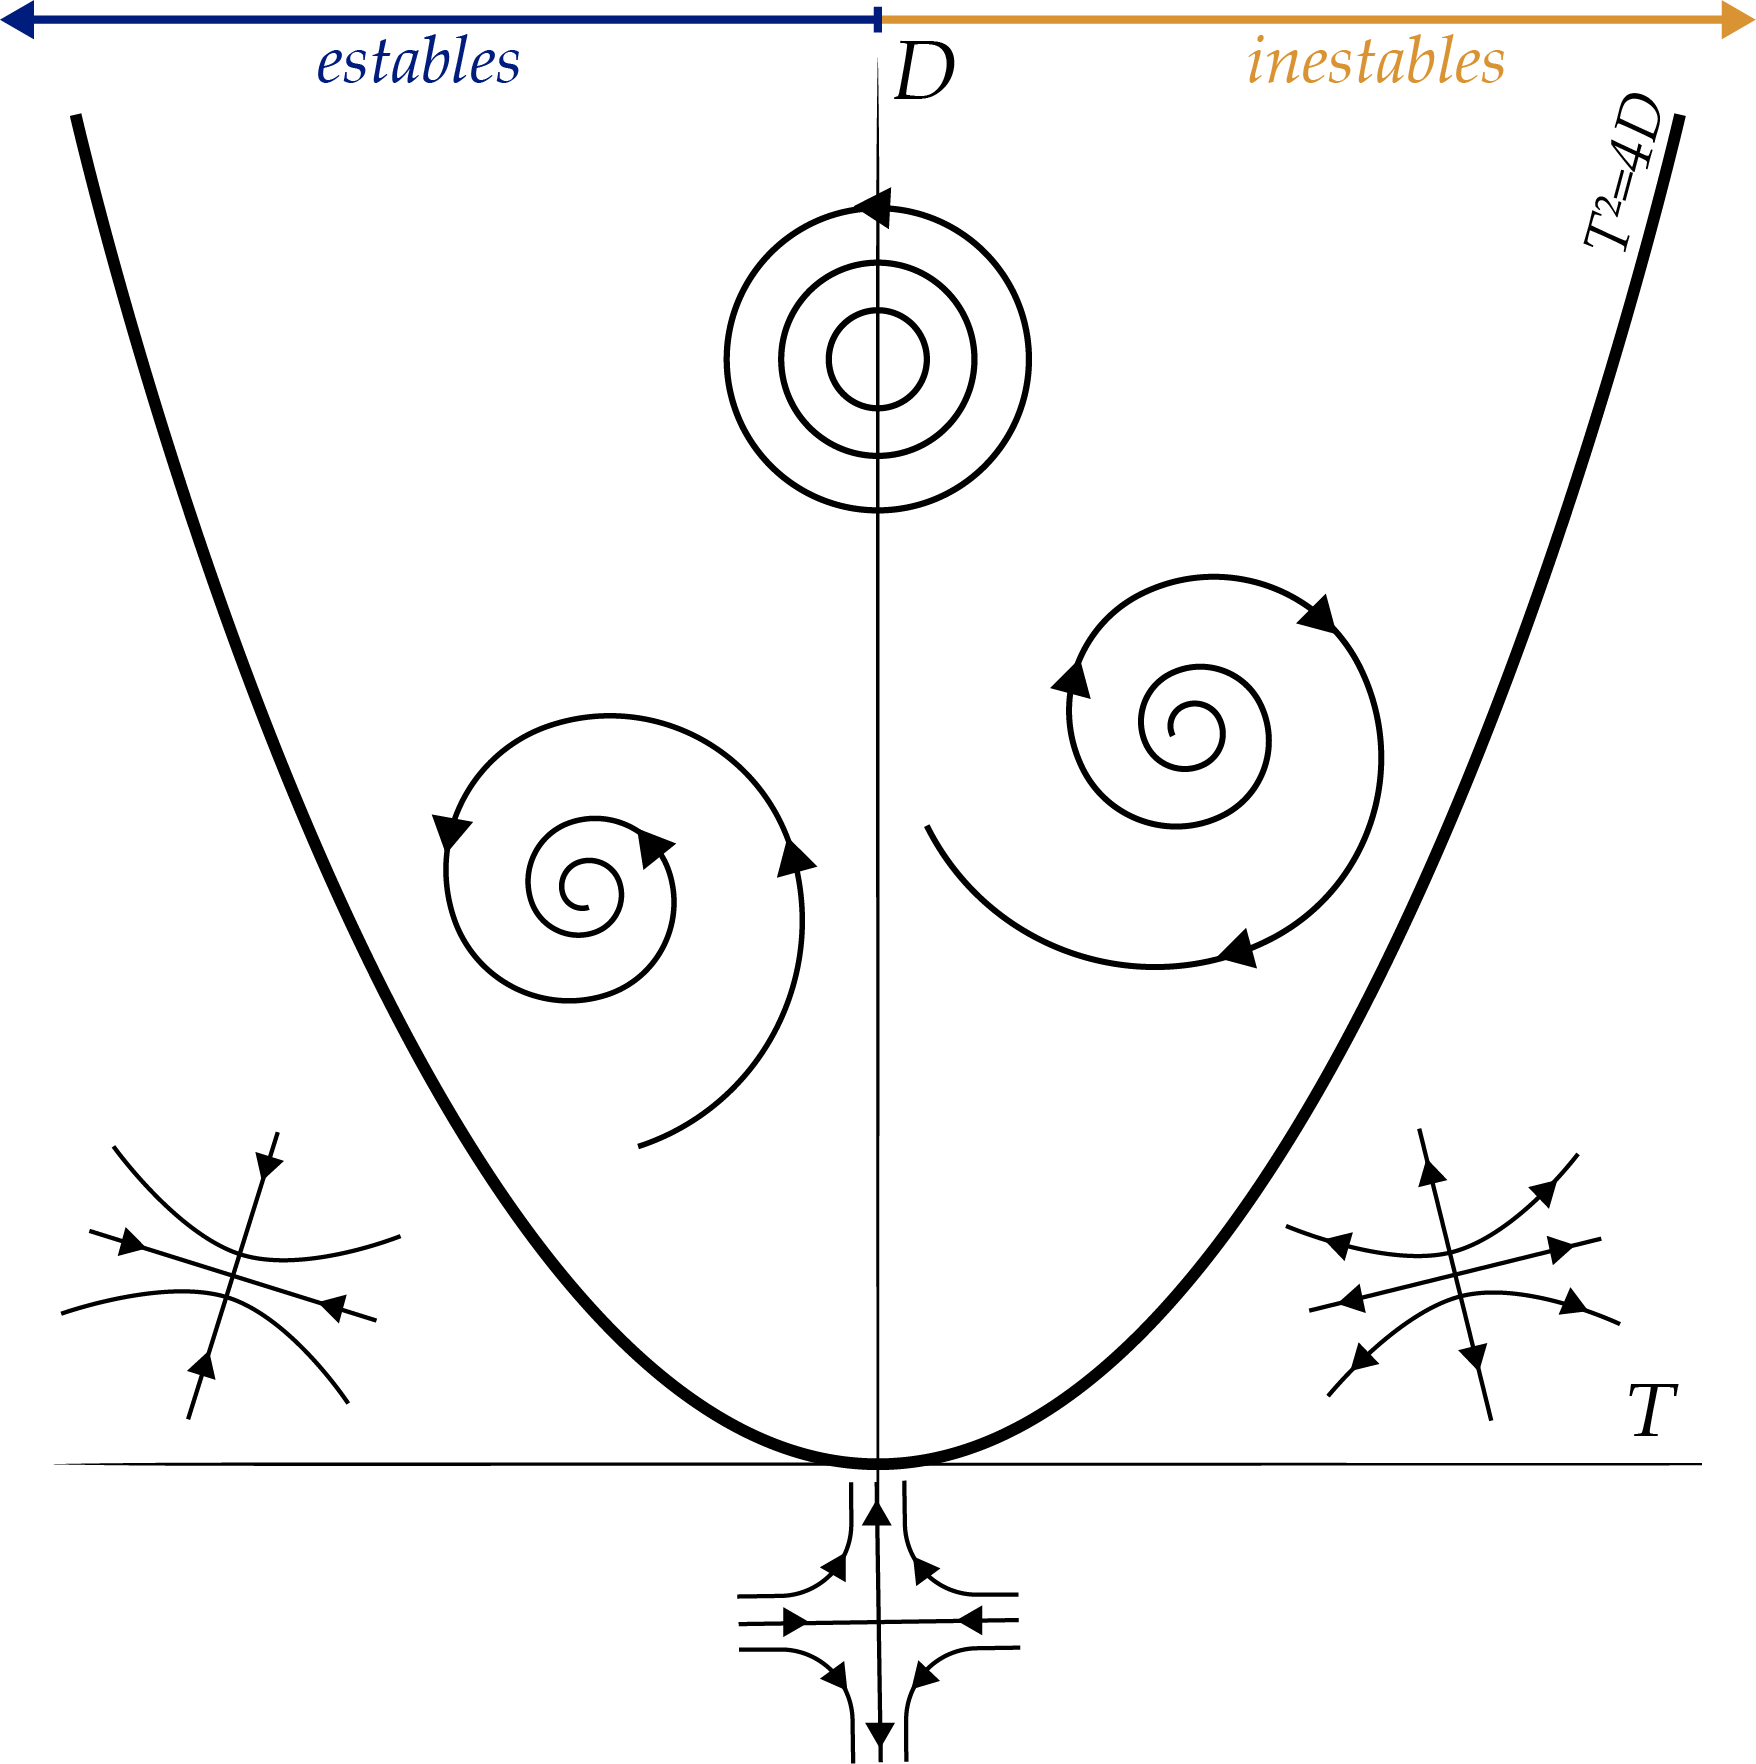
\includegraphics{6-resumen-puntos.png}
    \end{center}
\end{pro}
\begin{proof}
    Se sigue de forma directa de la introducción de esta subsección.
\end{proof}
%%%%%%%%%%%%%%%%%%%%%%%%%%%%%%%%%%%%%%%%%%%%%%%%%%%%%%%%%%%%%%%% Clase del 10/04
\begin{pro}[Relación de puntos críticos con el sistema lineal asociado]
    Si $(x_0, y_0)$ es un punto crítico propio de $\mathcal{SI}$, es decir:
    $$
        \mathrm{det}\mx{f_x(x_0, y_0) & f_y(x_0, y_0) \\ g_x(x_0, y_0) & g_y(x_0, y_0)} \neq 0
    $$
    entonces el aspecto de las trayectorias de $\mathcal{SI}$ cerca de $(x_0, y_0)$ es el mismo que el del sistema lineal asociado $\mathcal{SL}$ em $(0, 0)$ \textbf{salvo} en los casos:
    \begin{itemize}
        \item $\lambda_1 = \lambda_2 \neq 0$
        \item $Re(\lambda_i) = 0$, $(Im(\lambda_i) \neq 0)$.
    \end{itemize}
\end{pro}
\begin{obs}
    No se proporciona demostración de la proposición pero vamos a hacer algunos comentarios.
    \begin{itemize}
        \item En el caso $\lambda_1 = \lambda_2$ puede quedarse igual o convertirse en el aspecto de un $\lambda_1 \neq \lambda_2$, la estabilidad o no permanece.
        \item En el caso $Re = 0$, es decir $\lambda_i$ es un complejo puro, se puede quedar igual (centro), o pasar a un comportamiento en espiral (estable o inestable).
    \end{itemize}
\end{obs}

\begin{eg}[Análisis de puntos críticos. Sistema de presa/depredador simple.] \label{eg:centr-centr}
    Si quisiéramos modelizar las poblaciones de presa($x$) y depredador($y$) podríamos expresarlo por medio del sistema:
    $$
        \begin{cases}
            x' = 2x - \frac{1}{2}xy = f(x, y)\\
            y' = -3y + 5xy = g(x, y)
        \end{cases}
    $$
    Vamos a analizar los puntos críticos.\\
    Resolvemos:
    $$
        \begin{cases}
        f = x(2-\frac{y}{2}) = 0\\
        g = y(-3+5x) = 0
        \end{cases}
    $$
    De $f$ hallamos $x=0$ o $y = 4$, y de $g$ hallamos $y = 0$ o $x = \frac{3}{5}$. Así que los puntos críticos son:
    $(0, 0)$ y $(\frac{3}{5}, 4)$.\\
    Ahora calculamos:
    $$
        f_x = 2 - \frac{1}{2}y,\ f_y = -\frac{x}{2},\ g_x = 5y,\ g_y = -3+5x
    $$
    Y por tanto, la matriz de la aproximación lineal $\mx{f_x(x_0, y_0) & f_y(x_0, y_0) \\ g_x(x_0, y_0) & g_y(x_0, y_0)}$ queda en $(\frac{3}{5}, 4)$:
    $$
        \mx{0 & \frac{-3}{10}\\ 20 & 0} \leadsto \lambda = \pm \sqrt{6}i
    $$
    y por tanto es un centro en la aproximación lineal. Queremos saber que ocurre en el sistema original.\\
    La ecuación de las trayectorias:
    $$
        \dd{y}{x} = \frac{g}{f} = \frac{y(-3+5x)}{x(2-\sfrac{y}{2})}
    $$
    que es de variables separables y tras resolverla llegamos a:
    $$
        y^2x^3 = \pm e^C e^5x e^{\frac{y}{2}}
    $$
    y escogiendo el signo en función de $x$ para que preserve el valor absoluto obtendríamos:
    $$
        y^2 e^{-\frac{y}{2}} = k \frac{e^{5x}}{x^3}
    $$
    Y al representarlo veríamos que es una curva cerrada. Para dibujar las trayectorias puede ayudarnos dibujar el campo vectorial asociado al problema.\\
    Consideramos entonces el campo vectorial definido por la aplicación $h:\R^2 \to \R^2$ que lleva $(x, y)$ a $(f(x, y), g(x, y))$.\\\\
    Las curvas en las que $h$ es horizontal son aquellas en las que $g(x, y) = 0$, de la misma forma $h$ es vertical si $f(x, y) = 0$. Con esto hallamos donde están los vectores puramente verticales u horizontales, y para dar sentido a los vectores simplemente calculamos su valor de $h$.
    \begin{center}
        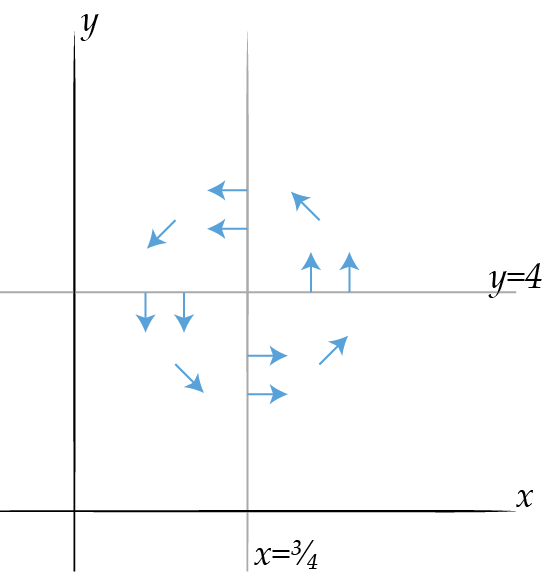
\includegraphics{6-campo-vectorial-presa.png}
    \end{center}
    %%%%%%%%%%%%%%%%%%%%%%%%%%%%%%%%%%%%%%%%%%%%%%%%%%%%%%%%%%%% Clase del 11/04
    Además del campo vectorial, que nos permite esbozar las trayectorias, podemos dibujarlas directamente a partir de la ecuación implícita de las mismas. Para ello vamos a usar que $ q \equiv y^2 e^{-\frac{y}{2}} = k \frac{e^{5x}}{x^3} \equiv p$, y vamos a representar en cada cuadrante una función distinta, $y$ frente a $x$ en el primer cuadrante, $q$ frente a $y$ en el segundo, $q$ frente a $p$ en el tercero y $p$ frente a $x$ en el cuarto.
    \begin{center}
        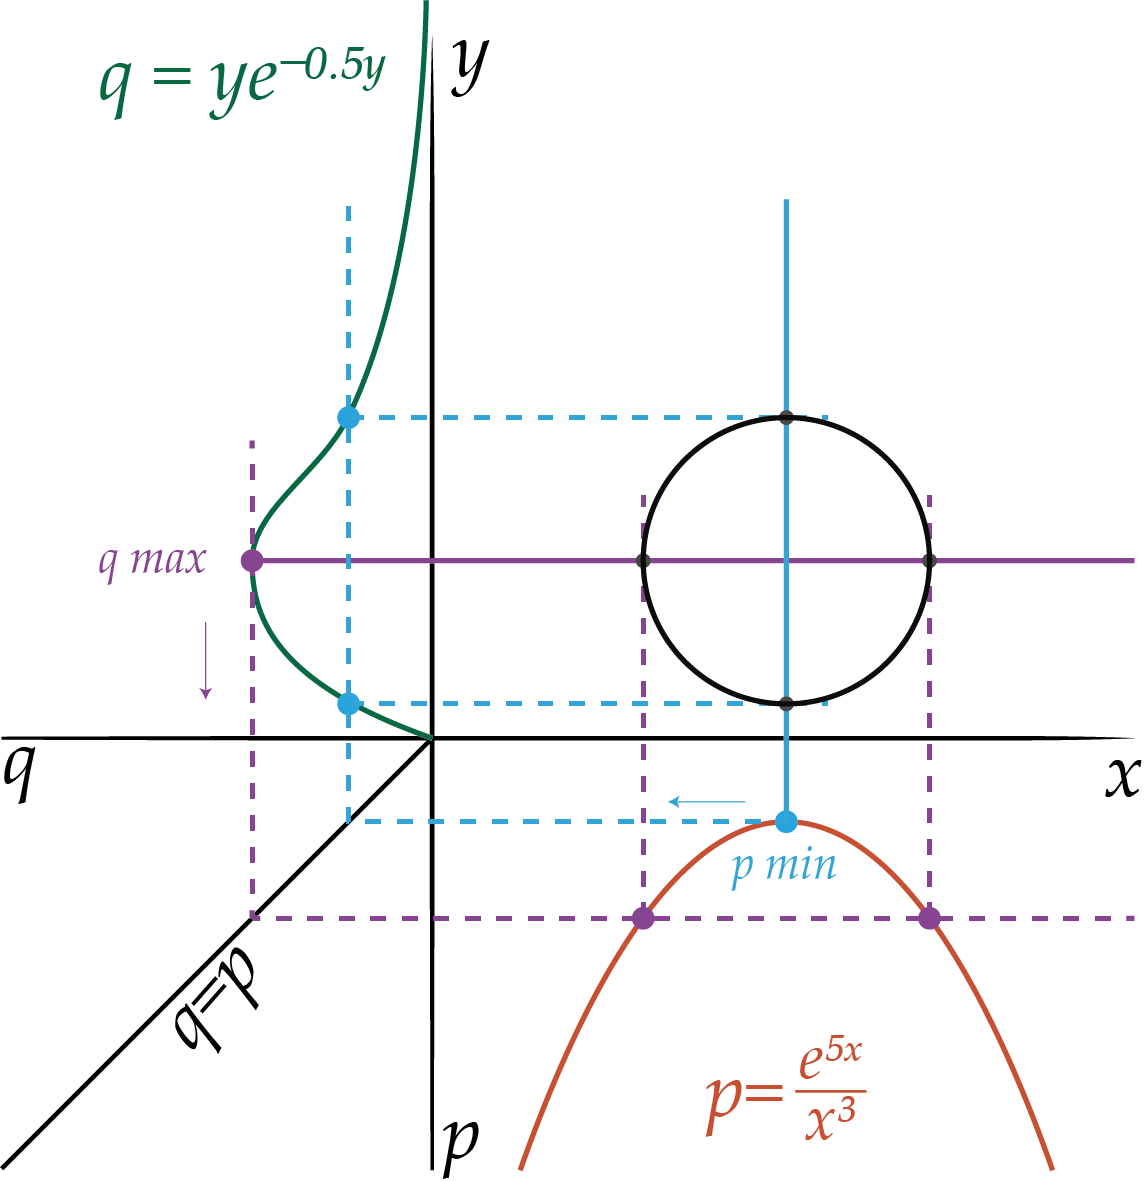
\includegraphics{6-trayectoria-presa.png}
    \end{center}
    Y en este caso vemos que el centro del sistema lineal es también un centro en el sistema original.
\end{eg}
\begin{th_ex}
    Prueba analíticamente que las trayectorias del ejemplo anterior son curvas cerradas.
\end{th_ex}
\begin{eg}[Sistemas con centro en sistema lineal pero espirales en el original]\label{eg:centr-esp}
    Sean los sistemas:
    $$
        \mathcal{I} =
        \begin{cases}
                x' = -y -x(x^2 + y^2)\\
                y' = x  - y(x^2 + y^2)
        \end{cases}
    $$
    $$
        \mathcal{II} =
        \begin{cases}
                x' = -y + x(x^2 + y^2)\\
                y' = x  + y(x^2 + y^2)
        \end{cases}
    $$
    Comparten el mismo sistema lineal:
    $$
        \mathcal{SL} =
        \begin{cases}
                x' = -y\\
                y' = x
        \end{cases}
    $$
    que expresado de forma matricial en $(0, 0)$ tiene como matriz de coeficientes: $\mx{0 & -1 \\ 1 & 0}$. Usando el criterio de traza y determinante podemos determinar fácilmente que es un centro. Sin embargo, podríamos ver que el $(0,0)$ de $\mathcal{I}$ es una espiral estable y en $\mathcal{II}$ es una espiral inestable.\\
    Para verlo analíticamente pasamos a polares y estudiamos la ecuación para $r(t)$. Visualmente podemos representar el campo vectorial de los sistemas originales con lo que veríamos como se comportan ambas espirales. Se deja al lector.
\end{eg}
\begin{obs}
    Como hemos visto, en los ejemplos \ref{eg:centr-esp} y \ref{eg:centr-centr} hallábamos un centro en el sistema lineal pero se puede transformar en espirales o seguir siendo un centro en el sistema original.
\end{obs}
\pagebreak %%XXX: This might fuck up later
\begin{eg}[Sistema de poblaciones competitivas con limitación de recursos compartidos.]
    Sea el sistema:
    $$
        \begin{cases}
            x' = x(2-x) - xy \equiv f\\
            y' = y(3-y) -2xy \equiv g
        \end{cases}
    $$
    Entonces la matriz del sistema lineal en cada punto crítico $(x_0, y_0)$ es:
    $$
        \mx{f_x(x_0, y_0) & f_y(x_0, y_0)\\ g_x(x_0, y_0) & g_y(x_0, y_0)}
    $$
    Los puntos críticos son los que cumplen que $f = g = 0$ y obtenemos para cada punto su matriz lineal y su interpretación con el criterio de la traza y el determinante:
    \begin{gather*}
        \text{P1: }(0, 0)\ \ \mx{2 & 0 \\ 0 & 3}\ \equiv \text{ nodo inestable.}\\
        \text{P2: }(0, 3)\ \ \mx{-1 & 0 \\ -6 & -3}\ \equiv \text{ nodo asintóticamente estable.}\\
        \text{P3: }(2, 0)\ \ \mx{-2 & -2 \\ 0 & -1}\ \equiv \text{ nodo asintóticamente estable.}\\
        \text{P4: }(1, 1)\ \ \mx{-1 & -1 \\ -2 & -1}\ \equiv \text{ punto de silla.}\\
    \end{gather*}
    Además, en los tres primeros puntos las trayectorias son tangentes al autovector $v_1$, de autovalor de menor tamaño (en valor absoluto).\\
    Los autovectores son:
    \begin{gather*}
        \text{P1: } v_1 = \mx{1\\ 0},\ v_2 = \mx{0\\1}\\
        \text{P2: } v_1 = \mx{1\\ -3},\ v_2 = \mx{0\\1}\\
        \text{P3: } v_1 = \mx{-2\\ 1},\ v_2 = \mx{1\\0}\\
        \text{P4: } v_1 = \mx{1\\ \sqrt{2}},\ v_2 = \mx{1\\-\sqrt{2}}\\
    \end{gather*}
    Entonces, en los puntos críticos podemos saber como van a comportarse la aproximación lineal de las trayectorias, que como no son ningún centro, tienen el mismo comportamiento que las trayectorias originales.
    Además, para seguir esbozando podemos trazar el campo vectorial $V$ sobre las curvas en las que o bien $f = 0$ o bien $g = 0$. Entonces, sea $V$:
    $$
        V = \mx{f\\g} = \mx{x(2-x-y)\\y(3-y-2x)}
    $$
    Estas curvas nos definen regiones en el espacio y siguiendo la dirección del campo vectorial podemos analizar a qué regiones vamos a poder volver o de cuales no vamos a poder salir.\\
    Se aporta una representación de las trayectorias en los puntos críticos y el campo vectorial en distintas regiones:
    \begin{center}
        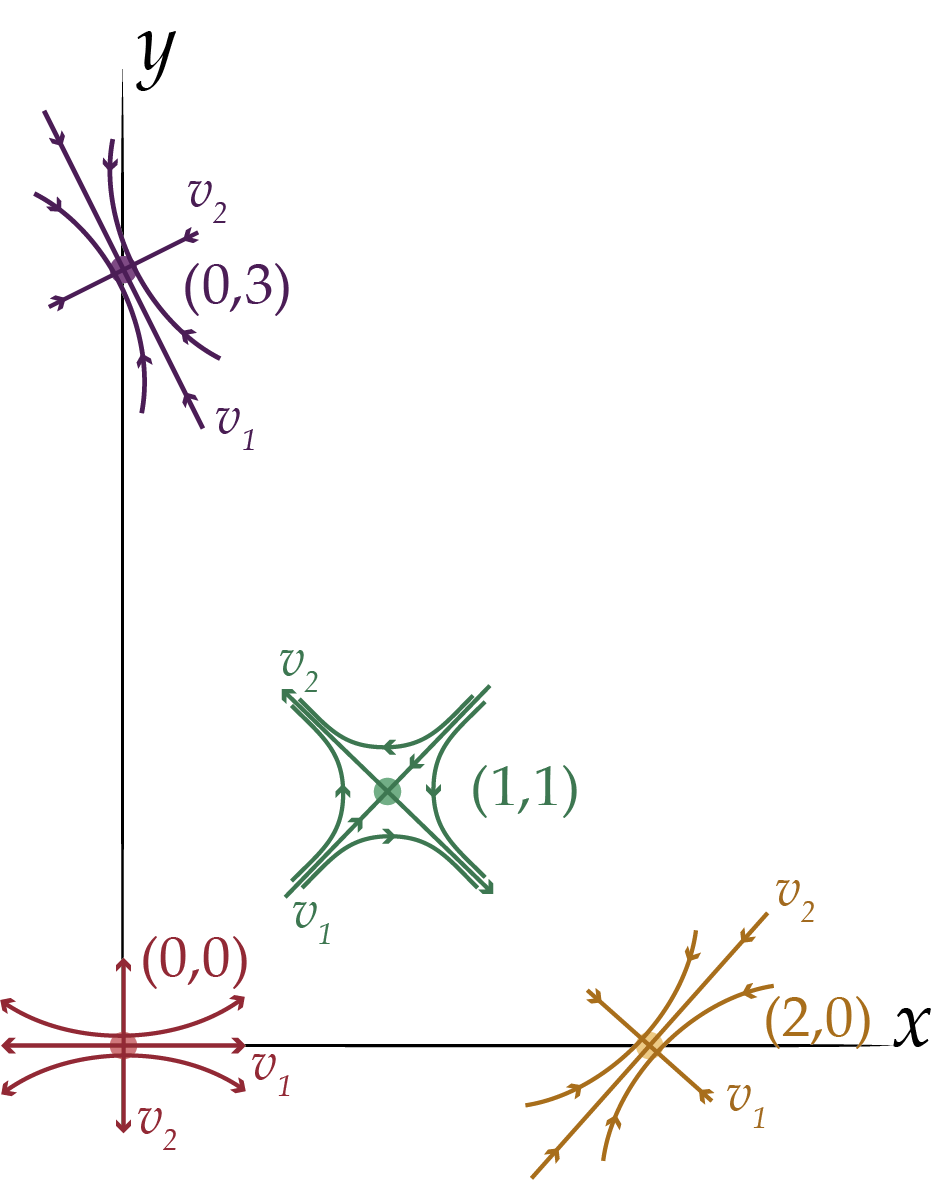
\includegraphics[width=0.45\textwidth]{6-aprox-lineal.png}
        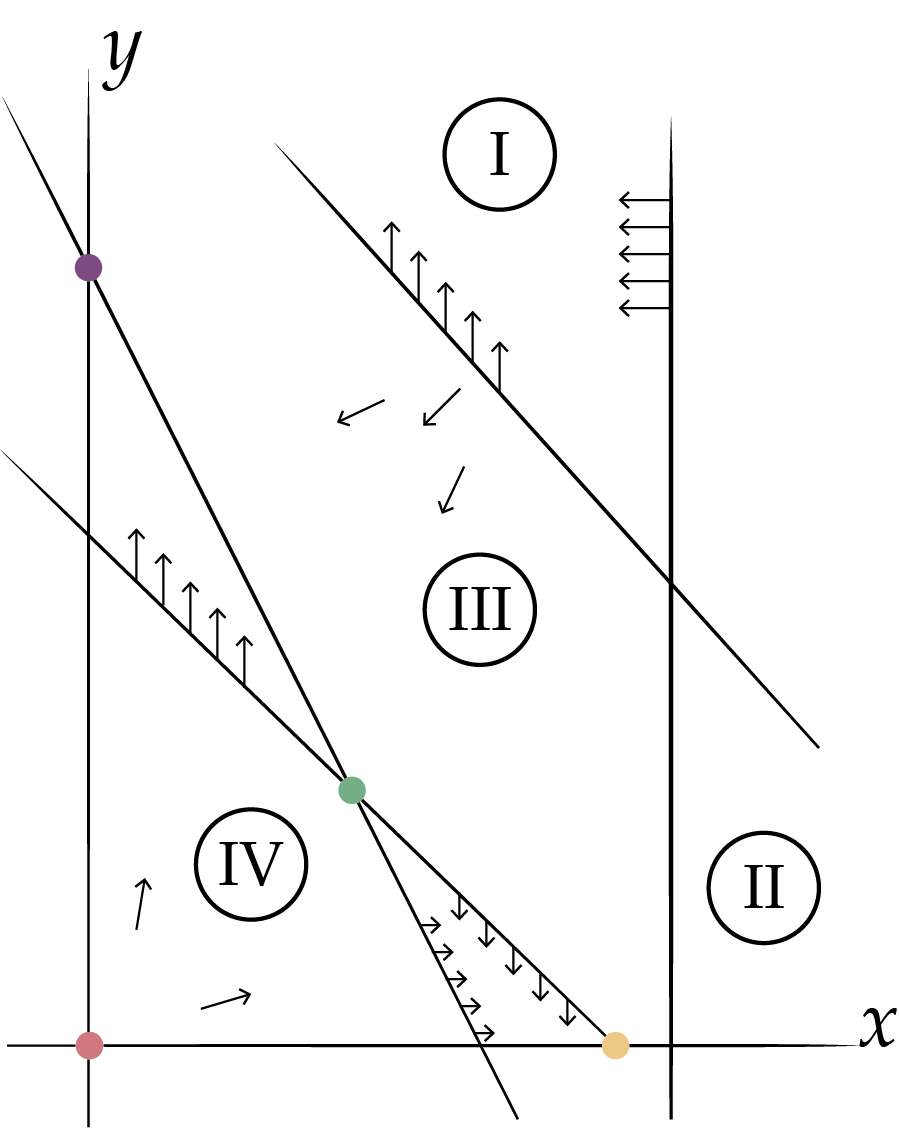
\includegraphics[width=0.45\textwidth]{6-campo-vectorial-regiones.png}
    \end{center}
\end{eg}
%%%%%%%%%%%%%%%%%%%%%%%%%%%%%%%%%%%%%%%%%%%%%%%%%%%%%%%%%%%%%%%% Clase del 23/04
%% TODO: Pedir a Santorum
%%%%%%%%%%%%%%%%%%%%%%%%%%%%%%%%%%%%%%%%%%%%%%%%%%%%%%%%%%%%%%%% Clase del 24/04
\section{Estabilidad de puntos críticos}
Consideraremos el sistema $\mathcal{S}$:
$$
    \mathcal{S} =
    \begin{cases}
        x' = f(x, y)\\
        y' = g(x, y)
    \end{cases}
$$
Y recordamos que $p = (x_0, y_0)$ es un punto crítico si $f(p) = g(p) = 0$.
\begin{dfn}[Punto crítico no singular]
    Diremos que un punto $p = (x_0, y_0)$ es singular en un sistema:
    $$
    \mathcal{S} =
    \begin{cases}
        x' = f(x, y)\\
        y' = g(x, y)
    \end{cases}
    $$ si y sólo si:
    $$
        \det \mx{f_x(p) & f_y(p)\\ g_x(p) & g_y(p)} = 0
    $$
\end{dfn}
Vamos a ver como estudiar la \textbf{estabilidad} de un punto crítico $p$ no-singular en $\mathcal{S}$.\\\\
Para los casos en que el $\mathcal{SL}$ sea el  sistema lineal asociado a $\mathcal{S}$ en $p$ tiene el mismo aspecto que el de $\mathcal{S}$ (es decir, la parte real de los autovalores es no nula), podemos concluir estabilidad en los casos pertinentes.
\begin{enumerate}
    \item Si $Re(\lambda_i) < 0,\ i\in\{1, 2\} \implies p$ estable
    \item Si un autovalor (al menos) tiene parte real $ > 0$, entonces es inestable.
\end{enumerate}
Sin embargo, en caso de que $Re(\lambda_i) = 0$, ya vimos que tenemos un centro para $\mathcal{SL}$, y que en el sistema original podemos tener o bien un centro o bien una espiral. En este caso vamos a ver un enfoque que mira directamente a $\mathcal{S}$.\\\\

Para realizar este análisis, vamos a intentar encontrar una función $E(x, y)$ que se comporte como una \textit{energía} en la que $p$ es \textbf{el} punto de \textit{energía mínima}, y tal que la \textit{energía} se mantiene o decrece a lo largo de las trayectorias cercanas a $p$.
\begin{dfn}[Signo de definición de una función]
    Sea $p = (x_0, y_0)$ un punto crítico para $\mathcal{S}$ y sean $f, g \in C^1$ en un entorno de $p$.\\
    Sea una función $E \in C^1$, $E(p) = 0$ y además:
    $$
        \exists r_0 > 0\ tq\ E: \B(p, r_0) \to \R
    $$
    Entonces, sea $q \neq p$ diremos que $E$ es:
    \begin{enumerate}
        \item \textbf{definida positiva} si y sólo si $E(q) > 0$.
        \item \textbf{semidefinida positiva} si y sólo si $E(q) \geq 0$.
        \item \textbf{definida negativa} si y sólo si $E(q) < 0$.
        \item \textbf{semidefinida negativa} si y sólo si $E(q) \leq 0$.
    \end{enumerate}
\end{dfn}
\begin{obs}
    Vamos a dar algunos ejemplos de funciones definidas positivamente:
    \begin{enumerate}
        \item $E(x, y) = x^2 + y^2$ es definida positiva para $(0,0)$
        \item $E(x, y) = \mx{x & y} \mx{\alpha & \beta \\ \beta & \gamma} \mx{x \\ y}$, es definida positiva si la matriz $2 \times 2$ lo es.
    \end{enumerate}
\end{obs}
Las funciones de \textit{energías} que comentábamos anteriormente son las funciones definidas positivamente para $p$. Además, la \textit{energía} se mantiene o decrece en las trayectorias. ¿En que se convierte esta idea?\\\\
$$
    \text{Sea } e(t) = E(x(t), y(t))
$$
Diremos que la energía se mantiene o decrece si: $\Dd{t} e(t) \leq 0$. Por tanto, desarrollando con la regla de la cadena obtenemos:
$$
    \dd{e}{t} = E_x(x(t), y(t)) x'(t) + E_y(x(t), y(t)) y'(t) = (E_x f + E_y g) (x(t) + y(t)) \leq 0
$$
Y para que esto se cumpla basta que $E_x f + E_y g \leq 0$ para cualquier punto $(x, y)$ cerca de $p$.

\begin{pro}[Estabilidad]\label{pro:establ}
    Si existe $E$ una función definida positiva en $p$, y además $E_x f + E_y g$ es semidefinida negativa en $p$ con $(E \in C^2)$, entonces $p$ es \textbf{estable} para $\mathcal{S}$.\\\\

    Recordemos que un punto $p$ es estable si:
    $$
        \forall \varepsilon > 0,\ \exists \delta > 0 : ||(x(t_0),y(t_0)) - p|| < \delta
    $$
    entonces:
    $$
        ||(x(t), y(t)) - p||< \varepsilon\ \forall t \geq t_0
    $$
\end{pro}
\begin{proof}
    Sea $ E: \B(p, r_0) \to \R$. Dado $\varepsilon > 0$, vamos a ver que exista un $\delta$ como en el enunciado. Podemos suponer $\varepsilon < r_0$.
    \begin{enumerate}
        \item Sea $m = \min_{\delta \B(p_0, \varepsilon)}$, que existe por ser $E$ continua y $\delta \B(p_0, \varepsilon)$ un compacto, y $m>0$ pues $E$ solo se anula en $p$ y es $>0$ fuera, en particular en la frontera de $\B$ (por ser definida positiva).
        \item $E(p) = 0$ y continua $\implies \exists \delta > 0$ tal que $E(q) < m$ si $||q - p|| < \delta$.
%%%%%%%%%%%%%%%%%%%%%%%%%%%%%%%%%%%%%%%%%%%%%%%%%%%%%%%%%%%%%%%% Clase del 25/04
        \item Si $(x(t_0), y(t_0)) \in \B(p, \delta)$ entonces $(x(t), y(t)) \in \B(p, \varepsilon)\ \forall t > t_0$, vamos a ver esto.\\\\
        Si fuera falso, esto querría decir que:
        $$
            \exists \bar{t} > t_0 : (x(\bar{t}), y(\bar{t})) \in \B(p, \varepsilon)
        $$
        y por tanto:
        $$
            e(\bar{t}) = E(x(\bar{t}), y(\bar{t})) \geq m
        $$
        Por otro lado:\\\\
        \begin{itemize}
            \item $e(t_0) \leq \frac{m}{2}$
            \item $\dd{e}{t} = E_x f + E_y g \leq 0$\\
            Por tanto, $e(t)$ decrece y $e(t) \leq e(t_0) \leq \frac{m}{2} < m\ \forall t \leq t_0$
        \end{itemize}
        Y como hemos visto que $e(t) \geq m$ y $e(t) < m$, entonces tenemos una contradicción lo hemos probado.
    \end{enumerate}
\end{proof}
\begin{dfn}[Función de Lyapunov débil]\label{pro:establ-asin}
    Una función como $E$ en la proposición \ref{pro:establ} se denomina \textbf{función de Lyapunov débil} para un sistema $\mathcal{S}$ (como al comienzo de la sección) en $p$.
\end{dfn}
\begin{pro}[Estabilidad asintóica]
    Si en las hipótesis del resultado de la proposición \ref{pro:establ} cambiamos $E_x f + E_y g$ semidefinida negativa por definida negativa entonces $p$ es asintóticamente estable, es decir:
    $$
        \exists \delta_0  (x(t_0), y(t_0)) \in \B(p, \delta_0) \implies (x(t), y(t)) \text{ converge a $p$ cuando } t \to +\infty
    $$
\end{pro}
\begin{proof}
    Tomamos $\varepsilon_0$ tal que las hipótesis sobre $E$, $E_x f + E_y g$ se cumplen en $\bar{\B}(p, \varepsilon_0)$. Por la proposición anterior:
    $$
        \exists \delta_0 : (x(t_0), y(t_0)) \in \B(p, \delta_0) \implies (x(t), y(t)) \in \B(p, \varepsilon_0)
    $$
    Con $e(t)$ como antes, $e(t) \downarrow 0$ cuando $t \to +\infty$ pues de lo contrario pasaría lo siguiente:
    \begin{itemize}
        \item $e(t)$ decrece.
        \item Si $e(t)$ no converge a $0$ entonces la trayectoria se queda en un anillo.
        \item Como $E_x f + E_y g$ es continua, no se anula en el anillo y es $< 0$ en él (pues es definida negativa), entonces:
        $$
            \exists r>0 : E_x f + E_y g \leq - \delta  0 \text{ en el anillo}
        $$
        Entonces si $t > t_0$:
        $$
            e(t) = e(t_0) + \int_{t_0}^{t} \dd{e}{t}(s) \d s \leq e(t) - \gamma(t-t_0) \downarrow -\infty \text{ cuando } t\to +\infty
        $$
    \end{itemize}
\end{proof}
\begin{dfn}[Función de Lyapunov fuerte]
    Una funcion $E$ como en la proposición \ref{pro:establ-asin} se llama \textbf{función de Lyapunov fuerte}
\end{dfn}
\subsection{Interpretación geométrica}
%% TODO: Añadir dibujos del 25/04

\begin{th_ex}
    Usando las mismas ideas, en especial que $e(t) = e(t_0) + \int_{t_0}^t \dd{e}{t}(s) \d s$, donde $\dd{e}{t} = E_x f + E_y g$, demostrar que si suponemos que $E$ está definida en todo $\R^2$ y cumple las hipótesis de la proposición \ref{pro:establ-asin} y además $E(q) \to +\infty$ entonces todas las trayectorias convergen a $p$.
\end{th_ex}
\begin{eg}
    Encontrar $\alpha$ tal que $x^2 + \alpha y^2$ es una función de Lyapunov (fuerte) en el punto $(0, 0)$ para el sistema:
    $$
        \begin{cases}
            x' = y - \sin^3(x)\\
            y' = -4x -\sin^3(y)
        \end{cases}
    $$
    \texttt{Analizamos la matriz del sistema lineal asociado}\\\\
    La matriz del sistema lineal asociado tiene como matriz: $\mx{0 & 1 \\ -4 & 0}$, que tiene autovalores $\pm \sqrt{2i}$ y por tanto es un centro. Como es un centro en el sistema lineal asociado, no podemos asegurar que lo sea en el sistema original, ya que podría ser un centro o una espiral (estable o inestable).\\\\
    \texttt{Hacemos un análisis más en profundidad del sistema original}\\\\
    Cuando $\alpha > 0 \implies x^2 + \alpha y^2$ es definida positiva. Además:
    $$
        E_x f + E_y g = 2x(y-\sin^3(X)) + 2\alpha y(-4x + \sin^3(y)) = (2 - 8\alpha) xy - 2x \sin^3(x) - 2 \alpha y \sin^3(y)
    $$
    Como $\sin^3(x) \sim x^3$ y $\sin^3(y) \sim y^3$ cerca de $(0,0)$, entonces basta encontrar un $\alpha$ tal que $2 - 8\alpha = 0 \implies \alpha = \frac{1}{4}$. Por tanto:
    $$
        E_x f + E_y g = -2x^4 \left(\frac{sen(x)}{x}^3\right) - \frac{1}{2}y^4 \left(\frac{sen(y)}{y}^3\right)
    $$
    y de nuevo, como $\frac{\sin(u)}{u} \sim 1$ cerca de $u = 0$, tenemos:
    $$
        E_x f + E_y g \leq -c (x^4 + y^4)
    $$
    Que es definida negativa y por tanto, hemos hallado el $\alpha$ que hace que la función $E$ sea una función de Lyapunov fuerte.
\end{eg}
%%%%%%%%%%%%%%%%%%%%%%%%%%%%%%%%%%%%%%%%%%%%%%%%%%%%%%%%%%%%%%%% Clase del 29/04
\begin{obs}
    Veamos algunas observaciones sobre el ejemplo anterior:\\
    \begin{enumerate}
        \item Si el comportamiento se corresponde con: %%TODO: Añadir dibujo
             el punto es inestable. Es decir:\\
             Si $E$ es definida positiva en $p$ y $E_x f + E_y g$ definida positiva en $p$ entonces $<\nabla E, V> > 0$ lo que implica que las trayectorias se alejan.\\\\
             Sin embargo, esto es pedir demasiado para que el punto sea inestable, de hecho, lo anterior solo recoge el caso del nodo inestable, donde todas las trayectorias se alejan del punto. Bastaría pedir que $E \in C^1$ y que $E_x f + E_y g > 0$ en $\R$.
        \item Si existe una curva cerrada simple tal que $V = \mx{f\\ g}$ apunta hacia dentro, entonces las trayectorias permanecen en la región delimitada por la curva.
    \end{enumerate}
\end{obs}
\section{Trayectorias cerradas}
En esta sección vamos a ver ciertos resultados sobre trayectorias cerradas de un sistema de ecuaciones. Es decir, las que corresponden a soluciones periódicas. Vamos a considerar el sistema:
$$
    \mathcal{S} =
    \begin{cases}
        x' = f(x, y)\\
        y' = g(x, y)
    \end{cases} \text{ con } f, g \in C^1 \text{ en una bola abierta de } \R^2
$$
\begin{pro}[Criterio de Bendixson]\label{pro:bendixson}
    Sea $\Omega \in \R^2$ es abierto, conexo y simplemente conexo. Si $(f_x + g_y)(x, y) \neq 0\ \forall (x, y) \in \Omega$, entonces no existe ninguna trayectoria cerrada de $\mathcal{S}$ que esté completamente contida en $\Omega$.
\end{pro}
\begin{proof}
    Vamos a demostrarlo por reducción al absurdo. Supongamos que existe dicha trayectoria $C = (x(t), y(t))$ cerrada y por tanto, una solución periódica. $C$ tiene que ser una curva cerrada simple, y por estar definida en $\R^2$ define una región $R$ en su interior.
    \begin{enumerate}
        \item Afirmamos que:
            $$
                \int_R (f_x + g_y) \d x \d y \neq 0
            $$
            Como $(f_x + g_y)$ continua, y $R\in \Omega$ es conexo, entonces $f_x + g_y$ no se anula en $R$, y por tanto $(f_x + g_y)$ no cambia de signo y la integral no se anula.
        \item Además:
            $$
                \int_C (f \d y - g \d x) = \pm \int_R (f_x + g_y) \d x \d y \neq 0
            $$
        \item La integral de línea sobre $C = (x(t), y(t))\ (periodica)$ es:
            $$
                \int_C f \d y - g \d x = \int_0^T (f(x(t), y(t))) y'(t) \d t - g(x(t), y(t)) x'(t) \d t = \int_0^T (fg - gf) \d t = 0
            $$
            Con lo que llegamos a la contradicción que estábamos buscando.
    \end{enumerate}
\end{proof}
%%%%%%%%%%%%%%%%%%%%%%%%%%%%%%%%%%%%%%%%%%%%%%%%%%%%%%%%%%%%%%%% Clase del 30/04
%\begin{eg}[Péndulo amortiguado]
%    Sea la EDO $x'' = -sen(x) - a x'$ con $a > 0$ que describe un péndulo con rozamiento, que corresponde al sistema:
%    $$
%        \begin{cases}
%            x' = y\\
%            y' = -sen(x) - ay
%        \end{cases}
%    $$
%    Entonces, podemos que ver que $f_x + g_y = -a < 0$.
%\end{eg}
\begin{obs}
    Se puede dar una versión del criterio de Bendixson (proposición \ref{pro:bendixson}) más general pero igual de difícil de aplicar.\\
    Si $h(x, y)$ no se anula, las trayectorias de:
    $$
        \begin{cases}
            x' = f\\
            y' = g
        \end{cases} \text{ y }
        \begin{cases}
            x' = hf\\
            y' = hg
        \end{cases}
    $$
    son las mismas.\\
    Eso quiere decir que en las condiciones del criterio, si $\exists h \in C^1$ que no se anula en $\Omega$ y $(hf)_x + (hf)_y$ tampoco se anula, y por tanto el sistema no tiene trayectorias cerradas contenidas en $\Omega$.
\end{obs}
\begin{pro}[Poincaré - Bendixson]\label{pro:poincare-bendixson}
    Sean $f, g \in C^1(\Omega)$, $\Omega$ dominio región en $\R^2$ abierto y conexo. Sea el sistema:
    $$
        \mathcal{S} =
        \begin{cases}
            x' = f(x, y)\\
            y' = g(x, y)
        \end{cases}
    $$
    Entonces:
    \begin{enumerate}
        \item Si $\Omega$ es simplemente conexo y $C \subset \Omega$ es una trayectoria cerrada, entonces $C$ \textit{encierra} un punto crítico de $\mathcal{S}$
        \item Sea $R \subset \Omega$ cerrado y acotado, tal que:\\
            \begin{itemize}
                \item $R$ no contiene puntos críticos de $\mathcal{S}$
                \item existe una trayectoria $C$ que comienza en $R$ y se mantiene en $R$, es decir tenemos una solución de $\mathcal{S}$ que cumple:
                $$
                    (x(t), y(t)) \in R \forall t : t_0 \leq t < \infty
                $$
            \end{itemize}
            Entonces ocurre una de las siguientes cosas:
            \begin{itemize}
                \item $C$ es una trayectoria cerrada.
                \item $C$ converge en espiral a una trayectoria cerrada (que se denomina ciclo límite)
            \end{itemize}
    \end{enumerate}
\end{pro}
\begin{proof}
    Vamos a ver la idea subyacente en la demostración en ambos resultados, la demostración escapa de los contenidos del curso.
    \begin{itemize}
        \item Siguiendo las figuras, $V$ es tangente a $C$ pues es una solución del sistema. Podemos ver como cambia la dirección del vector $V$ conforme recorremos la curva. Si llevamos el vector $V$ al origen vemos que ha completado una vuelta.\\\\
        Si ahora tomamos una curva cerrada cualquiera dentro de $C$, ahora no tiene por que ser tangente a la nueva curva, pues no tiene por qué ser solución del sistema. Sin embargo, si lo llevamos al origen volvemos a ver que el vector a lo largo de la nueva curva completa una vuelta.\\\\
        Si vamos reduciendo la longitud de la curva cerrada, acabamos llegando a un punto crítico, pues no existe una dirección definida para dicho punto ya que a lo largo de la curva el vector sigue dando una vuelta.
        \item El candidato a trayectoria cerrada del segundo resultado es:
        $$
            L = \{ q \in R : \exists t_k \to \infty tq\ (x(t_k), y(t_k)) \to q \}
        $$
        Donde se denomina \textit{conjunto límite} de $C$. $L$ es la trayectoria cerrada.
    \end{itemize}
\end{proof}
\begin{obs}
    Vamos a ver una forma habitual de aplicar el segundo resultado de \ref{pro:poincare-bendixson}.\\\\
    Vamos a buscar una region $R$ tal que el vector $V = \mx{f \\ g}$ que nos indica hacia donde se mueven las trayectorias, tal que el vector $V$ siempre apunte hacia \textit{dentro} de la region $R$.
\end{obs}
%%%%%%%%%%%%%%%%%%%%%%%%%%%%%%%%%%%%%%%%%%%%%%%%%%%%%%%%%%%%%%%% Clase del 06/05
\begin{eg}
    Sea el sistema:
    $$
        \begin{cases}
            x' = y + \frac{x}{4} (1 - 2(x^2+y^2))\\
            y' = -x + \frac{y}{2} (1 - (x^2+y^2))
        \end{cases}
    $$
    %TODO: Pedir a Santorum
%%%%%%%%%%%%%%%%%%%%%%%%%%%%%%%%%%%%%%%%%%%%%%%%%%%%%%%%%%%%%%%% Clase del 07/05
    \texttt{Clasificación de puntos críticos}\\\\
    Hallamos que el único punto crítico es el $(0,0)$. Para hallar de qué tipo es, vemos el sistema lineal asociado en $(0,0)$ que es:
    $$
        \begin{cases}
            x' = y + \frac{x}{4}\\
            y' = -x + \frac{y}{2}
        \end{cases}
    $$
    donde la matriz del sistema es: $\mx{\sfrac{1}{4} & 1 \\ -1 & \sfrac{1}{2}}$.\\
    Si hallamos los autovalores vemos que son de la forma: $\alpha \pm i \beta,\ \alpha > 0$, que corresponde a una espiral inestable. Faltaría ver la orientación de la espiral\\\\
    \texttt{Comportamiento en las regiones definidas por las trayectorias cerradas}\\\\
    Para ver que ocurre en la region existente entre las dos trayectorias cerradas, vamos a expresar el sistema en coordenadas polares utilizando el cambio:
    \begin{gather*}
        r^2 = x^2 + y^2,\ \theta = \tan^{-1}\left(\frac{y}{x}\right)\\
        \begin{cases}
            rr' = xx' + yy'\\
            r^2\theta' = xy' - yx'
        \end{cases}\\
        \text{Nota: este cambio solo permite estudiar puntos no cercanos al origen}
    \end{gather*}
    Si sustituimos y desarrollamos todo acabamos obteniendo:
    $$
        \begin{cases}
            r' = \frac{r\cos^2(\theta)}{4} (1-2r^2)+ \frac{r\sin^2(\theta)}{2} (1-r^2)\\
            \theta' = -1 + \frac{\sin(\theta)\cos(\theta)}{4} = -1 + \frac{\sin(2\theta)}{8}
        \end{cases}
    $$
    Al hacer el cambio de coordenadas, podemos calcular de nuevo los puntos críticos $(r' = 0,\ \theta' = 0)$ y en este caso no hay pues $\theta' \leq \frac{-7}{8}$. Como el ángulo tiene derivada negativa, entonces $\theta$ va de $+ \infty$ a $-\infty$, y por tanto todas las trayectorias giran en sentido de las agujas del reloj. Tendríamos que analizar el valor de $r'$ para ver si la espiral es estable (el radio decrece) o inestable (el radio crece).
\end{eg}
\begin{eg}
    Sea el sistema en coordenadas polares:
    $$
        r' = r(1-r^2) [r^2 \sin^2(\theta) + (r^2\cos^2(\theta) -1 )^2]\\
        \theta' = r^2 \sin^2(\theta) + (r^2\cos^2(\theta) -1 )^2
    $$
    Se deja como ejercicio escribir el sistema en función de las variables $(x, y)$. Recordemos que $rr' = xx' + yy'$ y $r^2\theta' = xy' - yx'$.
    \texttt{Análisis de puntos críticos ignorando el origen}\\\\
    Como analizamos en coordenadas polares ignoramos el origen. Los puntos críticos son los que hacen que $r' = 0,\ \theta' = 0$. Vemos fácilmente que del factor de $r'$: $(1-r^2)$, hallamos los puntos $(1, \theta)$ y $(-1, \theta)$. Faltaría ver cuando se anula $\theta'$ es decir:
    $$
        r^2 \sin^2(\theta) + (r^2\cos^2(\theta) -1 )^2 = 0 \leadsto
            \begin{cases}
                r\sin(\theta) = 0\\
                (r\cos(\theta))^2 = 1
            \end{cases} \implies \theta = n\pi,\ r = \pm 1.
    $$
    Por tanto, los puntos críticos en $(r, \theta)$ son $(\pm 1, n \pi)$, que corresponden a $(-1, 0)$ y $(1, 0)$ en $(x, y)$. A estos añadimos el origen que puede ser un punto crítico en $(x, y)$ ya que el análisis en polares puede eliminarlo.

\end{eg}
